 

\chapter{Combining texture features for emotion classification}
\label{Ch_4}

\minitoc

% **************************** Define Graphics Path **************************

%____________________________________Introduction selection _____________________________________%
\section{Introduction}

Facial expression recognition is a rapidly growing research topic due to an increased interest in applications of human-computer interaction. As discussed in chapter 2, it has been studied extensively over the past decade, with much research concentrating on geometric features.  Appearance based methods have become more prominent recently \citep{mishra2015survey,kumari2016fusion,yuqian2016action} and here we investigate the use of the combination of three feature descriptors, Histograms of Gradients (HOG) \citep{dalal2005histograms}, Dense Speeded Up Robust Features (D-SURF) \citep{lowe2004distinctive,uijlings2010real} and Local Binary Patterns (LBP) \citep{ojala1996comparative} for more accurate classification.  We show that the combination gives a strong image descriptor. Classification with random forests, which embody natural feature selection, further allows us to find the location of the most important image descriptors.  

% Obtaining labelled data for training emotion classification algorithms costly and researchers are usually forced to resort to using emotions displayed by actors, such as the famous Karolinska Directed Emotional Faces (KDEF) database \citep{lundqvist1998karolinska}.  To obtain more realistic data, we have used citizen volunteers to label a subset of the Labelled Faces in the Wild \citep{huang2012learning} database with the emotion being displayed. We describe the collection of this emotional Labelled Faces in the Wild (eLFW) dataset and illustrate the performance of the texture-based classifiers on it.

In our proposed system, there are four main steps to extract and classify facial features: face detection, face alignment, facial texture feature extraction (LBP, HOG and D-SURF) and classification.
We hypothesise that a combination of texture features is more effective than a single feature alone, yielding better classifications. In our experiments, we tested two state of the art classifiers, random forests and support vector machines (SVM).
Our proposed system has two training phases: the first one uses random forests to locate the important facial regions by estimate feature importance. The second training phase is to produce the final model by training with the important features only. The model automatically locates the important facial regions, which makes the classification faster and more accurate by excluding unnecessary and noisy face regions.

Image preparation and preprocessing steps are described in section \ref{sec:preprocessing}. We describe the feature extraction and combination in section \ref{sec:Extraction+combination}. Section \ref{sec:BaslineRandomForest} shows the baseline classification results for each one of the three feature extraction methods (HOG, LBP and D-SURF) with the two datasets (KDEF and eLFW), and then examines the effects of the combining texture features. 
Section \ref{sec:importance_mask} discusses the feature size reduction by determining only the important features and image masking. After that, we show random forest classification results applying the important features regions. Evidence of the similarity between machine and human classification is provided in section \ref{sec:Comparison_citizen}.
Classification using SVMs is discussed in section \ref{sec:SVM}.

The difficulties encountered by people and machines in distinguishing expressions displaying fear, anger and sadness leads us to consider alternative classifiers.  So in section \ref{sec:weight-pairw-class}, we describe a  pairwise random forest classifier in which the pairwise classifiers have a weighted vote to determine the overall class. We show how to optimise the weights using an evolutionary algorithm and present results showing the efficacy of the method. Finally, conclusions are drawn in section \ref{sec:ch4_Summary}.  





%____________________________________ImageFeaturesExtraction selection _____________________________________%




\section{Image preprocessing}
\label{sec:preprocessing}
Image preprocessing is an important step to prepare images for feature extraction. Where the region-of-interest (ROI) is the face, we detect faces within the image to remove unwanted regions from images. Face alignment is then used to reduce the wide variety of face pose angles. Finally, all images are converted from RGB to grey scale.


\begin{figure}[tb]
	\centering
	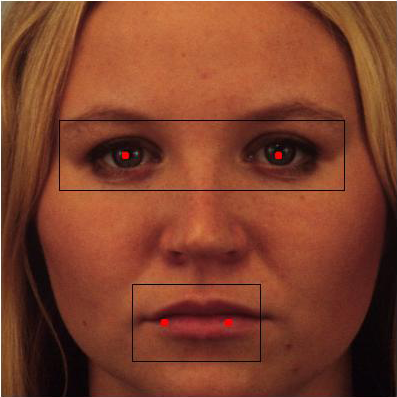
\includegraphics[width=50.5mm]{Chapter4/Figs/facePoints.png}
	\textbf{\caption{Facial points detection  }\label{fig:facePoints}}
\end{figure}

\begin{itemize}
	\item \textbf{Face detection and alignment}
	
	The first step is detecting the face. The face is detected using the Viola-Jones algorithm \citep{viola2004robust,viola2001rapid}.
	The Viola-Jones algorithm can find faces, mouths and eyes. Having located the face, to align it we need to estimate the main facial points from the centres of the eyes and two points over the mouth as shown in figure \ref{fig:facePoints}. Bounding boxes around the eyes and mouth are created by the Viola-Jones algorithm. We then calculate the centre points of the eyes and mouth in a similar manner to \citep{davison2014micro} these equations:
	
	\begin{equation}
	(Cl_{x}, Cl_{y}) = (\frac{W}{4} + x, \frac{H}{2} + y)
	\end{equation}
	
	
	\begin{equation}
	(Cr_{x}, Cr_{y}) = (\frac{3W}{4}  + x, \frac{H}{2} + y)
	\end{equation}
	
	where $Cl$ is the centre of the left eye, $Cr$ is the centre of the right eye, $W$ is the width of the bounding box, $H$  is the height, and $x$ and $y$ are the pixel locations of the top-left corner of the
	the bounding box for the eyes.
	
	
	
	All faces in the training dataset were aligned using the \cite{huang2012learning} method as shown in figure \ref{fig:aliegmen}. This alignment method depends on a combination between deep learning into the congealing alignment framework to obtain features that can represent the image at differing resolutions based on network depth. It use a  modified the learning algorithm for the restricted Boltzmann machine by combining a set sparsity penalty, which gives a topographic organization of the learned filters and improving subsequent alignment results \cite{huang2012learning}.
	
	 After alignment we estimated the face points, then we found the mean face shape by applying Procrustes analysis \citep{kendall1989survey}.  The detected points for each image face were aligned to the mean shape by affine transformation \citep{hazewinkel2001affine}, and each face was warped to its new aligned points.
	
	Figures \ref{fig:faceDetiction} and  \ref{fig:aliegmen} show an example of a detected and  face image after alignment and converting RGB values to grey then face detection.   
	
	
	%%%%%%%%%%%%%%%%%%%%%%%%%%%%%%%%%%%%%%%%%%%%%%%%%%%%%%%%%%%%%%%%%
	\begin{figure}[tb]
		\centering
		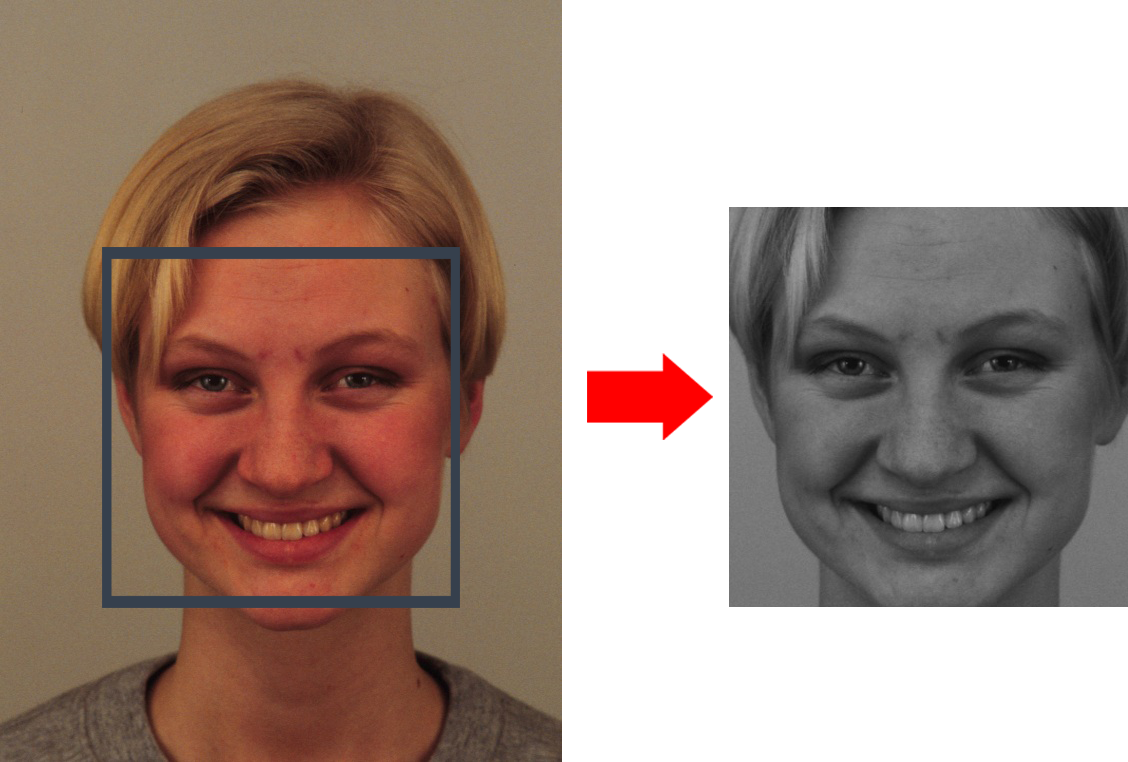
\includegraphics[width=60.5mm]{Chapter4/Figs/Face_Detection.png}
		\textbf{\caption{Face detection with Viola Jones  }\label{fig:faceDetiction}}
	\end{figure}
	%%%%%%%%%%%%%%%%%%%%%%%%%%%%%%%%%%%%%%%%%%%%%%%%%%%%%%%%%%%%%%%%%
	
	
	%%%%%%%%%%%%%%%%%%%%%%%%%%%%%%%%%%%%%%%%%%%%%%%%%%%%%%%%%%%%%%%%%
	
	%%%%%%%%%%%%%%%%%%%%%%%%%%%%%%%%%%%%%%%%%%%%%%%%%%%%%%%%%%%%%%%%%
	
	%%%%%%%%%%%%%%%%%%%%%%%%%%%%%%%%%%%%%%%%%%%%%%%%%%%%%%%%%%%%%%%%%
	\begin{figure}[tb]
		\centering
		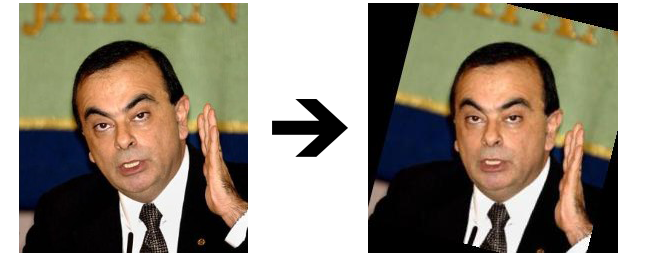
\includegraphics[width=55.5mm]{Chapter4/Figs/aliegmen.png}
		\textbf{\caption{An example of facial alignment .}\label{fig:aliegmen}}
	\end{figure}
	
	
	
	
	\item \textbf{Convert RGB image to greyscale.}
	
	Our proposed method works with greyscale images. LBP, HOG and D-SURF features were extracted from a greyscale image before classification.  All input images in the datasets we used are colour images. Converting RGB values to greyscale values by forming a weighted sum of the R, G, and B components: $0.2989 \times R + 0.5870 \times G + 0.1140 \times B$  \citep{kanan2012color}.
	
	%%%%%%%%%%%%%%%%%%%%%%%%%%%%%%%%%%%%%%%%%%%%%%%%%%%%%%%%%%%%%%%%%%
\end{itemize}
%
%
%\clearpage
%
%\newpage

\section{Texture-feature extraction and combination}
\label{sec:Extraction+combination}


%%%%%%%%%%%%%%%%%%%%%%%%%%%%%%%%%%%%%%%%%%%%%%%%%%%%%%%%%%%%%%%%%
\begin{figure}[tb]
	\centering
	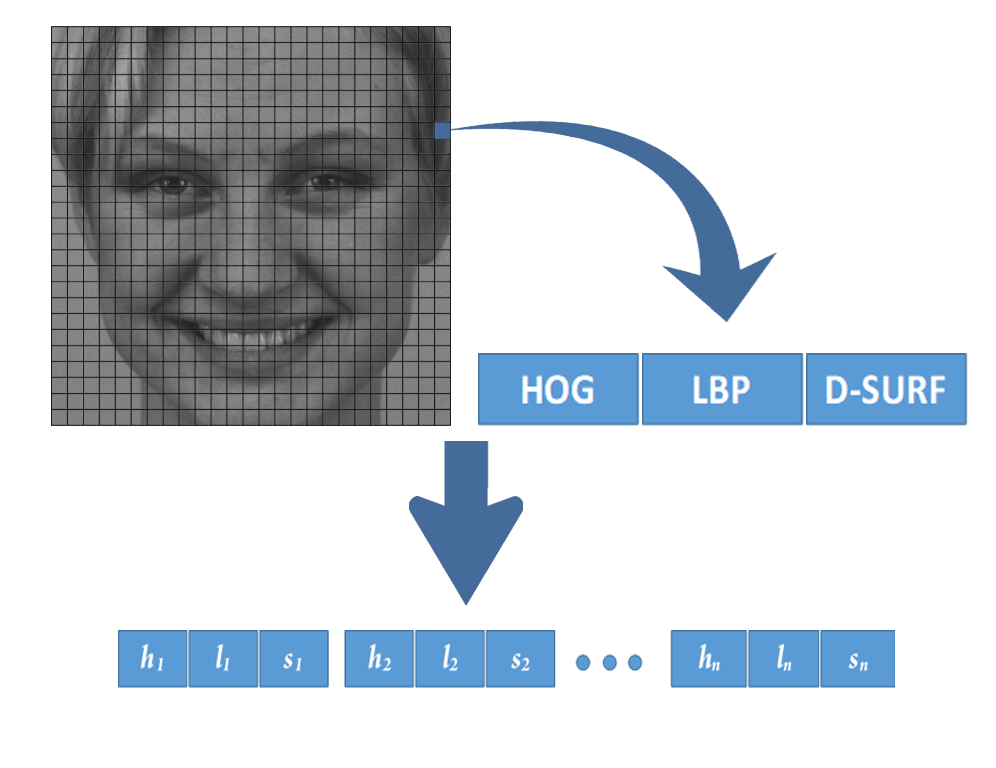
\includegraphics[width=0.6\textwidth]{Chapter4/Figs/HOGLBPSURF.png}
	\textbf{
		\caption{Block features (HOG, LBP and SURF) extraction and combination}
		\label{fig:HOGLBPSURF}}
\end{figure}
%%%%%%%%%%%%%%%%%%%%%%%%%%%%%%%%%%%%%%%%%%%%%%%%%%%%%%%%%%%%%%%%%


In machine learning and pattern recognition, feature extraction methods describe an image as a set of measured values called features.
This data may be useful for further processing such as in machine learning. In this thesis, we applied three commonly used image descriptors, Local Binary Pattern (LBP), Histogram of oriented gradients (HOG) and Dense Speeded Up Robust Features (D-SURF), where we hypothesise that a combination of the three descriptors would give better image description than any single one.  
Local binary pattern \citep{ojala1996comparative,ojala2002multiresolution} is a non-parametric descriptor which efficiently summarises the local structures of images.
%The LBP operator identifies each pixel of an image by decimal numbers, that encode the local structure neighbouring each pixel. Each pixel is compared with a three by three neighbourhood by subtracting the centre pixel value, which means eight neighbours. All pixels will be encoded 0 and 1.

For an image $\mathbf{I}$ with size 400 by 400, we divide it into 25 by 25 non-overlapping blocks, which means 625 blocks.  For each block the three feature descriptors: HOG $\mathbf{I_h}$, LBP $\mathbf{I_l}$ and D-SURF $\mathbf{I_s}$ are extracted and combined by concatenating each block's HOG, LBP and D-SURF descriptors in one vector $\mathbf{I_c} $.
%%%%%%%%%%%%%%%%%%%%%%%%%%%%%%%%%%%%%%%%%%%%%%%%%%%%%%%%%%%%%%%%%
\begin{equation}\label{eq:NoOfLBPCells}
\mathbf{I_c} = (\mathbf{I_{h_1}}  ,\mathbf{I_{l_1}} ,\mathbf{I_{s_1}} \mathbf{I_{h_2}}  ,\mathbf{I_{l_2}} ,\mathbf{I_{s_2}} , ... ,\mathbf{I_{h_n}}  ,\mathbf{I_{l_n}} ,\mathbf{I_{s_n}})
\end{equation}.
%%%%%%%%%%%%%%%%%%%%%%%%%%%%%%%%%%%%%%%%%%%%%%%%%%%%%%%%%%%%%%%%
 Figure \ref{fig:HOGLBPSURF} illustrates the division into blocks and feature extraction and combination.








The three features descriptors have been extracted for all the image blocks. The length of HOG for each block is $81$, for LBP is $9$ and for D-SURF is $64$. So the length of the concatenated features is $81+64+9= 154$, and for the image $154\times625=96250$.

%
% the extracted HOG features for the whole image is 50625 divided into 625 blocks with this and then the overall size $\times 625 = 50625 $. The LBP feature length is 5625 into 625 blocks, and each block length is . Each . The combined feature block length is  , and the whole image combined feature is  









% %____________________________________ masking selection _____________________________________%
%
%\section{Image masking and unwanted features reduction}
%\label{sec: masking}








%
%\clearpage
%\newpage
%

\section{Baseline Random Forest Classification}
\label{sec:BaslineRandomForest}

\subsection{KDEF experiments}
Initially,  we tested the performance of each one of the three features (HOG, LBP and D-SURF) separately with random forest classifier. 10-fold cross-validation was used ti classify the 490 images in the  KDEF data. The results are shown in tables \ref{KDEFwithHOGonly}, \ref{KDEFwithLBPonly} and \ref{KDEFwithD-SURFonly}. 
Table \ref{KDEFwithHOGonly} shows the confusion matrix with only the HOG feature; the overall accuracy was 73\%. Table \ref{KDEFwithLBPonly} shows the confusion matrix result with the LBP features, where the overall accuracy was 79.9\%. Finally, table \ref{KDEFwithD-SURFonly} shows the D-SURF result with an overall accuracy of 70.3\%. 


The combined features were also tested with Random Forests and 10-fold cross-validation as well. Table  \ref{table:RF_KDEF_compined} illustrates a visualisation of the performance. It is clear from the table that the combined model performance is emphatically better than using single one of the three features, achieving an overall accuracy of 89.8\%. 









%%%%%%%%%%%%%%%%%%%%%%%%%%%%%%%%%%%%%%%%%%%%%%%%%%%%%%%%%%%%%%%%%
\begin{table}[tb]
	\fontsize{12}{12}
	\centering    
	\textbf{
		\caption{Confusion matrix for  KDEF images with HOG featurs and a Random Forest classifier. True classes are shown by rows, with assigned classes in columns. The overall accuracy is 73\%.}\label{KDEFwithHOGonly}}

	\begin{tabular}{@{}|l|c|c|c|c|c|c|c|@{}}
		\hline
		& \textbf{FE}    & \textbf{AN}     & \textbf{DI}       & \textbf{HA}    & \textbf{NE}    & \textbf{SA}    & \textbf{SU}  \\ \hline
		\textbf{FE} & \textbf{0.299}  & 0.042          & 0.028             & 0.042          & 0.113          & 0.142          & 0.328        \\ \hline
		\textbf{AN} & 0.000           & \textbf{0.771} & 0.113             & 0.028          & 0.071          & 0.014          & 0.000        \\ \hline
		\textbf{DI} & 0.000           & 0.042          & \textbf{0.771}    & 0.085          & 0.0284         & 0.057          & 0.014        \\ \hline
		\textbf{HA} & 0.0142          & 0.014          & 0.000             & \textbf{0.914} & 0.057          & 0.000          & 0.00          \\ \hline
		\textbf{NE} & 0.000           & 0.099          & 0.000             & 0.000          & \textbf{0.842} & 0.028          & 0.028          \\ \hline
		\textbf{SA} & 0.042           & 0.099          & 0.                & 0.014          & 0.227          & \textbf{0.542} & 0.028          \\ \hline
		\textbf{SU} & 0.000           & 0.000          & 0.000             & 0.000          & 0.028          & 0.000               & \textbf{0.971}  \\ \hline
	\end{tabular}
\end{table}
%%%%%%%%%%%%%%%%%%%%%%%%%%%%%%%%%%%%%%%%%%%%%%%%%%%%%%%%%%%%%%%%%



%%%%%%%%%%%%%%%%%%%%%%%%%KDEFwithLBPonly%%%%%%%%%%%%%%%%%%%%%%%%%%%%%%%%%%
\begin{table}[H]
	\fontsize{12}{12}
	
	\centering    
	\textbf{
		\caption{Confusion matrix for  KDEF images with LBP features and Random Forests classifier. The overall accuracy is: 79.9\%.}\label{KDEFwithLBPonly}}
	
	
	\begin{tabular}{@{}|l|c|c|c|c|c|c|c|@{}}
		\hline
		& \textbf{FE}    & \textbf{AN}    & \textbf{DI}    & \textbf{HA}     & \textbf{NE}        & \textbf{SA}     & \textbf{SU}     \\ \hline
		\textbf{FE} & \textbf{0.456}  & 0.056          & 0.028          & 0.042           & 0.056              & 0.042           & 0.313           \\ \hline
		\textbf{AN} & 0.000           & \textbf{0.771} & 0.113          & 0.028           & 0.071              & 0.000           & 0.014           \\ \hline
		\textbf{DI} & 0.000           & 0.042          & \textbf{0.914} & 0.042           & 0.000              & 0.000           & 0.000           \\ \hline
		\textbf{HA} & 0.000           & 0.000          & 0.014          & \textbf{0.957}  & 0.028              & 0.000           & 0.000           \\ \hline
		\textbf{NE} & 0.000           & 0.028          & 0.000          & 0.000               & \textbf{0.942} & 0.000           & 0.028           \\ \hline
		\textbf{SA} & 0.028           & 0.028          & 0.042          & 0.085           & 0.142              & \textbf{0.628}  & 0.042          \\ \hline
		\textbf{SU} & 0.014           & 0.000          & 0.000          & 0.000           & 0.071              & 0.000           & \textbf{0.928}\\ \hline
	\end{tabular}
\end{table}
%%%%%%%%%%%%%%%%%%%%%%%%%%%KDEFwithLBPonly%%%%%%%%%%%%%%%%%%%%%%%%%%%%%%%%%%%%%





%%%%%%%%%%%%%%%%%%%%%%%%%%%%%KDEFwithD-SURFonly%%%%%%%%%%%%%%%%%%%%%%%%%%%%%%%%%%%%
\begin{table}[H]
	\fontsize{12}{12}
	\centering    
	\textbf{
		\caption{Confusion matrix for  KDEF photos with D-SURF features and Random Forests classifier. The overall accuracy is: 70.3\%.}\label{KDEFwithD-SURFonly}}
	\begin{tabular}{@{}|l|c|c|c|c|c|c|c|@{}}
		\hline
		& \textbf{FE}     & \textbf{AN}     & \textbf{DI}     & \textbf{HA}     & \textbf{NE}     & \textbf{SA}     & \textbf{SU}     \\ \hline
		\textbf{FE} & \textbf{0.214}     & 0.085          & 0.057          & 0.057          & 0.100           & 0.171           & 0.314          \\ \hline
		\textbf{AN} & 0.014              & \textbf{0.714} & 0.171          & 0.028          & 0.057           & 0.000           & 0.014         \\ \hline
		\textbf{DI} & 0.000              & 0.043          & \textbf{0.886} & 0.057          & 0.000           & 0.014           & 0.000           \\ \hline
		\textbf{HA} & 0.000              & 0.000          & 0.014          & \textbf{0.957} & 0.028           & 0.000           & 0.000            \\ \hline
		\textbf{NE} & 0.014              & 0.071          & 0.000          & 0.000          & \textbf{0.786}  & 0.000           & 0.128          \\ \hline
		\textbf{SA} & 0.028              & 0.057          & 0.057          & 0.142          & 0.171          & \textbf{0.442}  & 0.099         \\ \hline
		\textbf{SU} & 0.028             & 0.000          & 0.000          & 0.000          & 0.043           & 0.000           & \textbf{0.929}\\ \hline
	\end{tabular}
\end{table}
%%%%%%%%%%%%%%%%%%%%%%%%%%%%%%%%KDEFwithD-SURFonly%%%%%%%%%%%%%%%%%%%%%%%%%%%%%%%%%



\begin{table}[H]
	\fontsize{12}{12}
	\centering
	
	\caption{Confusion matrix for KDEF images with the combined features and Random Forests classifier. The overall accuracy is:  82.2\%. }
	\label{table:RF_KDEF_compined}
	\begin{tabular}{@{}|l|c|c|c|c|c|c|c|@{}}
		\hline
		& \textbf{FE}     & \textbf{AN}    & \textbf{DI}     & \textbf{HA} & \textbf{NE} & \textbf{SA}    & \textbf{SU}            \\ \hline
		\textbf{FE} & \textbf{0.657} & 0.129          & 0.043           & 0.000           & 0.014           & 0.100          & 0.057           \\ \hline
		\textbf{AN} & 0.000          & \textbf{0.829} & 0.100           & 0.000           & 0.000           & 0.057          & 0.014           \\ \hline
		\textbf{DI} & 0.000          & 0.057          & \textbf{0.871}  & 0.000           & 0.000           & 0.043          & 0.029           \\ \hline
		\textbf{HA} & 0.014          & 0.014          & 0.014           & \textbf{0.943}  & 0.000           & 0.014          & 0.000          \\ \hline
		\textbf{NE} & 0.000          & 0.000           & 0.014          & 0.071           & \textbf{0.886}  & 0.014           & 0.014              \\ \hline
		\textbf{SA} & 0.071          & 0.043          & 0.057           & 0.000           & 0.000           & \textbf{0.800}  & 0.029              \\ \hline
		\textbf{SU} & 0.157          & 0.029          & 0.029           & 0.000           & 0.000           & 0.014           & \textbf{0.771}   \\ \hline
	\end{tabular}
	
\end{table}












\subsection{eLFW experiments}
\label{sec:eLFWexperiments}

To test how the three texture features work with real rather then posed emotions. As before we evaluated the performance using single feature types. 10-fold cross-validation was used with 5000 Random forest trees for the 1310 eLFW faces. The results are shown in tables \ref{eLFWwithHOGonly}, \ref{eLFwithLBPonly} and \ref{eLFWwithD-SURFonly}. 
Table \ref{eLFWwithHOGonly} shows the confusion matrix eLFW database, and with only HOG feature, the overall accuracy was 73\%. Table \ref{eLFwithLBPonly} shows the confusion matrix result with LBP feature, where the overall accuracy was 60.9\%. Finally, table \ref{eLFWwithD-SURFonly} shows the D-SURF result with an overall accuracy of 51.2\% 


It is clear from this section that with the LBP, HOG and D-SURF it was hard to classify the fear expression where happy and neutral are more easily classified in both datasets and fear is most often misclassified. The combination of the three texture features improved the overall accuracy with both datasets.   

However, the overall accuracy for eLFW is lower than for KDEF, but the pattern of misclassification is the same, so it is clear the fear emotion for an instant was the lowest accuracy where the happy emotion was the higher for both dataset, KDEF and eLFW.



%%%%%%%%%%%%%%%%%%%%%%%%%%%eLFWwithHOGonly%%%%%%%%%%%%%%%%%%%%%%%%%%%%%%%%%%%%%%
\begin{table}[tb]
	\fontsize{12}{12}
	\centering    
	\textbf{
		\caption{Confusion matrix for eLFW images with HOG featurs and a Random Forest classifier. True classes are shown by rows, with assigned classes in columns. The overall accuracy is: 56.9\%.}\label{eLFWwithHOGonly}}
	
	\begin{tabular}{@{}|l|c|c|c|c|c|c|c|@{}}
		\hline
		& \textbf{FE}    & \textbf{AN}    & \textbf{DI}    & \textbf{HA}    & \textbf{NE}    & \textbf{SA}    & \textbf{SU}    \\ \hline
		\textbf{FE} & \textbf{0.137} & 0.158          & 0.195          & 0.058          & 0.084          & 0.184          & 0.184          \\ \hline
		\textbf{AN} & 0.092          & \textbf{0.608} & 0.067          & 0.025          & 0.042          & 0.042          & 0.125          \\ \hline
		\textbf{DI} & 0.069          & 0.044          & \textbf{0.681} & 0.063          & 0.044          & 0.050          & 0.050          \\ \hline
		\textbf{HA} & 0.036          & 0.039          & 0.036          & \textbf{0.742} & 0.070          & 0.036          & 0.048          \\ \hline
		\textbf{NE} & 0.042          & 0.054          & 0.071          & 0.083          & \textbf{0.638} & 0.046          & 0.054          \\ \hline
		\textbf{SA} & 0.150          & 0.130          & 0.085          & 0.030          & 0.035          & \textbf{0.465} & 0.105          \\ \hline
		\textbf{SU} & 0.086          & 0.043          & 0.029          & 0.057          & 0.043          & 0.071          & \textbf{0.671}\\ \hline
	\end{tabular}
\end{table}
%%%%%%%%%%%%%%%%%%%%%%%%%%eLFWwithHOGonly%%%%%%%%%%%%%%%%%%%%%%%%%%%%%%%%%%%%%%%




%%%%%%%%%%%%%%%%%%%%%%%%%eLFwithLBPonly%%%%%%%%%%%%%%%%%%%%%%%%%%%%%%%%%%
\begin{table}[H]
	\fontsize{12}{12}
	
	\centering    
	\textbf{
		\caption{Confusion matrix for eLFW images with LBP features and Random Forests classifier. The overall accuracy is: 60.9\%.}\label{eLFwithLBPonly}}
	
	
	\begin{tabular}{@{}|l|c|c|c|c|c|c|c|@{}}
		\hline
		& \textbf{FE}    & \textbf{AN}    & \textbf{DI}    & \textbf{HA}    & \textbf{NE}    & \textbf{SA}    & \textbf{SU}    \\  \hline
		\textbf{FE} & \textbf{0.184} & 0.153          & 0.195          & 0.047          & 0.074          & 0.179          & 0.168          \\ \hline
		\textbf{AN} & 0.092          & \textbf{0.650} & 0.058          & 0.017          & 0.033          & 0.033          & 0.117          \\ \hline
		\textbf{DI} & 0.069          & 0.044          & \textbf{0.719} & 0.050          & 0.038          & 0.038          & 0.044          \\ \hline
		\textbf{HA} & 0.027          & 0.033          & 0.036          & \textbf{0.773} & 0.045          & 0.036          & 0.048          \\ \hline
		\textbf{NE} & 0.025          & 0.033          & 0.050          & 0.079          & \textbf{0.729} & 0.042          & 0.042          \\ \hline
		\textbf{SA} & 0.150          & 0.125          & 0.075          & 0.020          & 0.025          & \textbf{0.500} & 0.105          \\ \hline
		\textbf{SU} & 0.114          & 0.071          & 0.057          & 0.057          & 0.043          & 0.071          & \textbf{0.586} \\ \hline
	\end{tabular}
\end{table}
%%%%%%%%%%%%%%%%%%%%%%%%%%%eLEFwithLBPonly%%%%%%%%%%%%%%%%%%%%%%%%%%%%%%%%%%%%%


%%%%%%%%%%%%%%%%%%%%%%%%%%%%%eLFWwithD-SURFonly%%%%%%%%%%%%%%%%%%%%%%%%%%%%%%%%%%%%
\begin{table}[tb]
	\fontsize{12}{12}
	\centering    
	\textbf{
		\caption{Confusion matrix for eLFW images with D-SURF features and Random Forests classifier. The overall accuracy is: 51.2\%.}\label{eLFWwithD-SURFonly}}
	\begin{tabular}{@{}|l|c|c|c|c|c|c|c|@{}}
		\hline
		& \textbf{FE}    & \textbf{AN}    & \textbf{DI}    & \textbf{HA}    & \textbf{NE}    & \textbf{SA}    & \textbf{SU}    \\ \hline
		\textbf{FE} & \textbf{0.168} & 0.153          & 0.195          & 0.058          & 0.079          & 0.179          & 0.168          \\ \hline
		\textbf{AN} & 0.100          & \textbf{0.508} & 0.067          & 0.092          & 0.050          & 0.058          & 0.125          \\ \hline
		\textbf{DI} & 0.081          & 0.056          & \textbf{0.656} & 0.075          & 0.050          & 0.038          & 0.044          \\ \hline
		\textbf{HA} & 0.042          & 0.039          & 0.045          & \textbf{0.645} & 0.100          & 0.052          & 0.076          \\ \hline
		\textbf{NE} & 0.042          & 0.054          & 0.058          & 0.079          & \textbf{0.650} & 0.063          & 0.054          \\ \hline
		\textbf{SA} & 0.155          & 0.145          & 0.085          & 0.060          & 0.040          & \textbf{0.375} & 0.140          \\ \hline
		\textbf{SU} & 0.114          & 0.086          & 0.057          & 0.114          & 0.100          & 0.114          & \textbf{0.414} \\ \hline
	\end{tabular}
\end{table}
%%%%%%%%%%%%%%%%%%%%%%%%%%%%%%%%eLFWwithD-SURFonly%%%%%%%%%%%%%%%%%%%%%%%%%%%%%%%%%





\begin{table}[H]
	\fontsize{12}{12}
	\centering
	
	\caption{Confusion matrix for eLFW images with the combined features and Random Forests classifier. The overall accuracy is: $67.3\%$}
	\label{Table:eLFW&Random}
	\begin{tabular}{@{}|l|c|c|c|c|c|c|c|@{}}
		\hline
		& \textbf{FE}     & \textbf{AN}    & \textbf{DI}    & \textbf{HA} & \textbf{NE} & \textbf{SA}    & \textbf{SU}            \\ \hline 
		\textbf{FE} & \textbf{0.232} & 0.153          & 0.184          & 0.026           & 0.079           & 0.168          & 0.158           \\ \hline 
		\textbf{AN} & 0.092          & \textbf{0.650} & 0.058          & 0.025           & 0.017           & 0.042          & 0.117           \\ \hline 
		\textbf{DI} & 0.063          & 0.044          & \textbf{0.738} & 0.050           & 0.038           & 0.038          & 0.031           \\ \hline 
		\textbf{HA} & 0.012          & 0.006          & 0.021          & \textbf{0.927}  & 0.024           & 0.003          & 0.006           \\ \hline 
		\textbf{NE} & 0.008          & 0.008           & 0.021          & 0.054           & \textbf{0.879}  & 0.017           & 0.013          \\ \hline 
		\textbf{SA} & 0.150          & 0.135          & 0.075          & 0.025           & 0.020           & \textbf{0.490}  & 0.105               \\ \hline 
		\textbf{SU} & 0.157          & 0.143          & 0.171          & 0.043           & 0.014           & 0.086           & \textbf{0.386}  \\ \hline 
	\end{tabular}
	
\end{table}







%
%\clearpage
%\newpage
\section{Feature importance mask}
\label{sec:importance_mask}
After the three type of features have been extracted and combined,
% then we excluded two blocks surrounding the image to be 25 by 25 blocks. The combined feature length was 81466, each combined block length 154.
The features of images are trained by random forests to estimate the predictor importance for each value of the combined feature vector; see chapter 2. Then each image block is matched with its part of the combined vectors to decide where the important facial parts are. To locate the important face part, we sum the importance values for each face block, to yield a matrix of 25 by 25 combined importance vales. We applied the Otsu method \citep{otsu1975threshold} to covert the importance values to binarise. A mask of size 25 by 25 was produced. After getting the mask, by bicubic interpolation, we resized it to 400 by 400 to be the same as the size of training and testing images. Figures \ref{fig:MaskinGiagram} and \ref{fig:impportSteps} illustrate the main steps of mask creation.

%%%%%%%%%%%%%%%%%%%%%%%%%%%%%%%%%%%%%%%%%%%%%%%%%%%%%%%%%%%%%%%%%
\begin{figure}[tb]
	\centering
	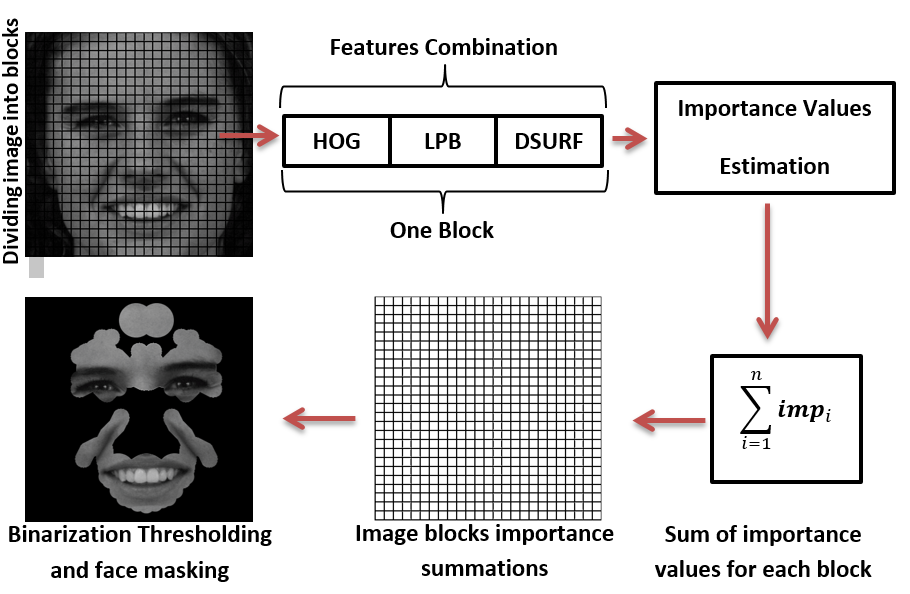
\includegraphics[width=0.5\textwidth]{Chapter4/Figs/MaskingDiagram.png}
	\textbf{
		\caption{Diagram of image importance masking }
		\label{fig:MaskinGiagram}}
\end{figure}
%%%%%%%%%%%%%%%%%%%%%%%%%%%%%%%%%%%%%%%%%%%%%%%%%%%%%%%%%%%%%%%%%


Figure \ref{fig:impportColours} illustrates how a comparison between the random forest importance prediction values. Red colours show that HOG features were the most important in the location, while green colour refers to LBP and blue to D-SURF. It is clear that HOG and LBP occupy most the facial region compared to D-SURF.   
%%%%%%%%%%%%%%%%%%%%%%%%%%%%%%%%%%%%%%%%%%%%%%%%%%%%%%%%%%%%%%%%%
\begin{figure}[tb]
	\centering
	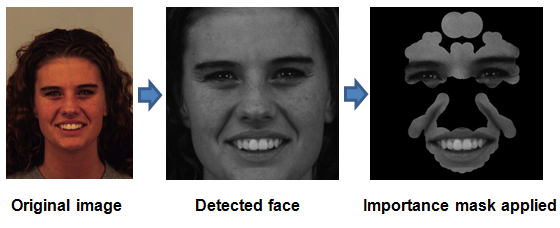
\includegraphics[width=0.9\textwidth]{Chapter4/Figs/maskingSteps.png}
	\caption{Importance masking steps for a KDEF image.}
	\label{fig:impportSteps}
\end{figure}
As Figure \ref{fig:KDEFandeLFW_masks} shows, this procedure identifies the eyes, mouth, creases at the side of the nose and the forehead as most informative. We point out that this is an empirically determined mask rather than one chosen \textit{a priori} and we obtain slightly different masks for the acted and wild faces. 

Table \ref{Table:eLFW&Random} and \ref{table:maskedeLFW} show two confusion matrices for that test, one with mask and one without. The accuracy on the eLFW data rose from $67.3\%$ to $71.6\%$ by using the importance mask. Fear and surprised expressions were the lowest accuracies. The model was still excellent with happy and neutral expression, and gave good results with anger and disgust, and acceptable with sad.


\section{Random forest classification with importance mask}
\label{sec:RF_mask}
After obtaining the masks from the two datasets KDEF and eLFW, we applied each mask to all images in each dataset to remove the unwanted parts and keep only those that were important. The resulting features were then  classified using random forest (5000 trees). 10-fold cross validation was used to evaluate the classification  scheme.



%%%%%%%%%%%%%%%%%%%%%%%%%%%%%%%%%%%%%%%%%%%%%%%%%%%%%%%%%%%%%%%%%
\begin{figure}[tb]
	\centering
	\begin{subfigure}{.4\textwidth}
		\centering
		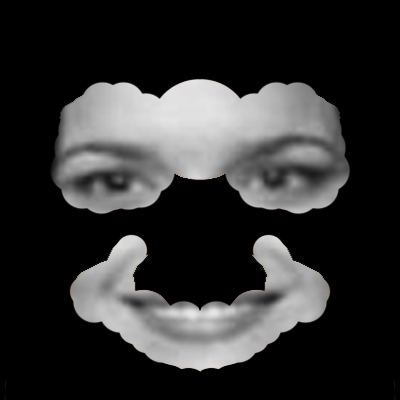
\includegraphics[width=.8\linewidth]{Chapter4/Figs/LWFmask.png}
		\caption{eLFW mask}
		\label{fig:LFWmask}
	\end{subfigure}%
	\begin{subfigure}{.4\textwidth}
		\centering
		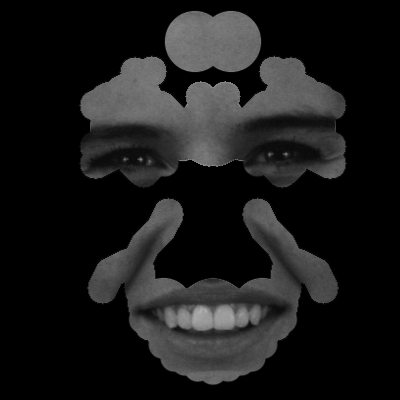
\includegraphics[width=.8\linewidth]{Chapter4/Figs/KDEFmask.png}
		\caption{KDEF mask}
		\label{fig:KDEFmask}
	\end{subfigure}
	\caption{Mask identifying the most important regions of the face for emotion classification derived by binarisng feature importance mas.}
	\label{fig:KDEFandeLFW_masks}
\end{figure}
%%%%%%%%%%%%%%%%%%%%%%%%%%%%%%%%%%%%%%%%%%%%%%%%%%%%%%%%%%%%%%%%%
\subsection*{KDEF experiments}

The table \ref{table:MASKED KDEF} shoes the confusion matrix for masked KDEF images with the combined features and Random Forests classifier. The overall accuracy is: $89.9\%$. The happy expression had the highest classification rate, while the fear expression had the lowest. With these two expressions, there is no significant improvement between masking and without masking.

%%%%%%%%%%%%%%%%%%%%%%%%%%%%%%%%%%%%%%%%%%%%%%%%%%%%%%%%%%%%%%%%%
\begin{table}[H]
	\fontsize{12}{12}
	
	\centering    
	\textbf{
		\caption{Confusion matrix for masked KDEF images with the combined features and Random Forests classifier. The overall accuracy is: $89.9\%$.}\label{table:MASKED KDEF}}
	
	\begin{tabular}{@{}|l|c|c|c|c|c|c|c|@{}}
		\hline
		& \textbf{FE}      & \textbf{AN}    & \textbf{DI}    & \textbf{HA} & \textbf{NE} & \textbf{SA}    & \textbf{SU} \\ \hline
		\textbf{FE}  & \textbf{0.671}   & 0.143          & 0.043          & 0.000           & 0.000           & 0.143          & 0.000 \\ \hline
		\textbf{AN}  & 0.000            & \textbf{0.857} & 0.071          & 0.000           & 0.000           & 0.071          & 0.000 \\ \hline
		\textbf{DI}  & 0.000            & 0.043          & \textbf{0.929} & 0.000           & 0.000           & 0.029          & 0.000 \\ \hline
		\textbf{HA}  & 0.000            & 0.000          & 0.000          & \textbf{0.986}  & 0.014            & 0.000         & 0.000 \\ \hline
		\textbf{NE}  & 0.000            & 0.000          & 0.000          & 0.014           & \textbf{0.986}  & 0.000          & 0.000 \\ \hline
		\textbf{SA} & 0.043              & 0.029         & 0.043          & 0.000           & 0.000           & \textbf{0.886} & 0.000 \\ \hline
		\textbf{SU} & 0.014              & 0.000         & 0.014          & 0.000           & 0.000           & 0.000          & \textbf{0.971} \\ \hline
	\end{tabular}
	
\end{table}
%%%%%%%%%%%%%%%%%%%%%%%%%%%%%%%%%%%%%%%%%%%%%%%%%%%%%%%%%%%%%%%%

%%%%%%%%%%%%%%%%%%%%%%%%%%%%%%%%%%%%%%%%%%%%%%%%%%%%%%%%%%%%%%%%%
\begin{table}[H]
	\centering
	\caption{Comparison of classification accuracy of random forest classification using masked LBP, HOG and D-SURF texture features with other recent techniques.  Evaluation on the KDEF data.}
	\label{table:us-vs-others}
	\begin{tabular}{@{}ll@{}}
		\toprule
		Method     \hspace{5.8cm}               & Accuracy   \tabularnewline   \midrule
		\cite{rao2015multi}                    & 74.05\%    \tabularnewline
		\cite{santra2016local}                 &  83.51\%   \tabularnewline
		\cite{santra2016saliency}              &  84.07\%  \tabularnewline 
		\cite{yuqian2016action}                & 88.7\%    \tabularnewline
		Random forests with masked texture features          & 89.8\%    \tabularnewline  
		Pairwise weighted random forests with masked texture features (\S \ref{sec:weight-pairw-class})         & 95.1\%    \tabularnewline  \bottomrule
		
	\end{tabular}
\end{table}
%%%%%%%%%%%%%%%%%%%%%%%%%%%%%%%%%%%%%%%%%%%%%%%%%%%%%%%%%%%%%%%%%

The neutral and surprise rose significantly by applying the mask, $88.6\%$  to $98.6\%$ for neutral, and  $77.1\%$  to $97.1\%$ for the surprise expression.
Table \ref{table:us-vs-others} demonstrates that when evaluated on the KDEF data our proposed method using random forest classifiers and masked LBP, HOG and D-SURF features compares favourably with other state of the art techniques.  



%%%%%%%%%%%%%%%%%%%%%%%%%%%%%%%%%%%%%%%%%%%%%%%%%%%%%%%%%%%%%%%%%
\begin{figure}[tb]
	\centering
	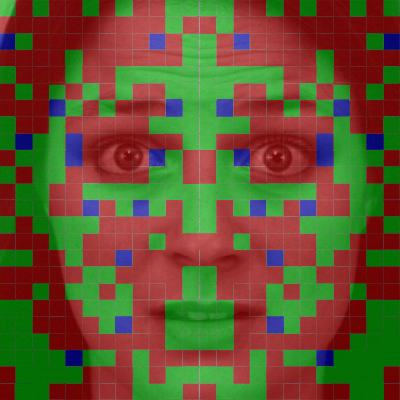
\includegraphics[width=50.0mm]{Chapter4/Figs/colours1.png}
	\caption{HOG, LBP and SURF importance values comparison.Red, blue and green indicate which feature type (HOG, LBP and D-SURF) was most important for each block. }
	\label{fig:impportColours}
\end{figure}
%%%%%%%%%%%%%%%%%%%%%%%%%%%%%%%%%%%%%%%%%%%%%%%%%%%%%%%%%%%%%%%%%







%%%%%%%%%%%%%%%%%%%%%%%%%%%%%%%%%%%%%%%%%%%%%%%%%%%%%%%%%%%%%%%%%
\begin{table}[tb]
	\fontsize{12}{12}
	\centering
	\textbf{
		\caption{Confusion matrix on eLFW database using proposed method, trained with KDEF.  Overall accuracy was $74.7\%$.}\label{eLFWwithKDEF}}
	\begin{tabular}{@{}|l|c|c|c|c|c|c|c|@{}}
		\hline
		& \textbf{FE}    & \textbf{AN}    & \textbf{DI}    & \textbf{HA} & \textbf{NE} & \textbf{SA}    & \textbf{SU}    \\ \hline
		\textbf{FE} & \textbf{0.371} & 0.086          & 0.114             & 0.043           & 0.043       & 0.071         & 0.271    \\ \hline
		\textbf{AN} & 0.057     & \textbf{0.643} & 0.157          & 0.000           & 0.014            & 0.057            & 0.071     \\ \hline
		\textbf{DI} & 0.43    & 0.029          & \textbf{0.743}   & 0.000           & 0.071            & 0.014            & 0.100     \\ \hline
		\textbf{HA} & 0.029   & 0.014          & 0.000            & \textbf{0.929}  & 0.014            & 0.014            & 0.000     \\ \hline
		\textbf{NE} & 0.014   & 0.014          & 0.014            & 0.029           & \textbf{0.900}   & 0.014            & 0.014     \\ \hline
		\textbf{SA} & 0.029   & 0.014          & 0.043            & 0.000           & 0.029            & \textbf{0.871}   & 0.014       \\ \hline
		\textbf{SU} & 0.157   & 0.014          & 0.043            & 0.000           & 0.000             & 0.014           & \textbf{0.771} \\ \hline
	\end{tabular}
\end{table}
%%%%%%%%%%%%%%%%%%%%%%%%%%%%%%%%%%%%%%%%%%%%%%%%%%%%%%%%%%%%%%%%%
\subsection*{eLFW experiments}
Importance masks are slightly different according to the training data images, so when we trained the system with KDEF photos, the mask was as shown in figure \ref{fig:impportSteps}. The eLFW training produced a mask with some differences as shown in figure \ref{fig:KDEFandeLFW_masks}.


Table \ref{table:maskedeLFW} shows a confusion matrix for masked eLFW images. It is clear that apply the mask significantly increased the accuracy from $67.3\%$  without masking to $71.6\%$ with masking (see table \ref{Table:eLFW&Random}). The happy and neutral expressions are most easily classified in both datasets and fear is most often misclassified, particularly in the eLFW data, where it is confused with all the other classes except happy and neutral. 




    




%\subsection*{KDEF Mask}
%
%\subsection*{eLFW Mask}








%%%%%%%%%%%%%%%%%%%%%%%%%%%%%%%%%%%%%%%%%%%%%%%%%%%%%%%%%%%%%%%%%%
%\begin{figure}[tb]
%\centering
%  \includegraphics[width=50 mm]{Chapter4/Figs/LFWmask.png}
%  \textbf{
%    \caption{}
%    \label{fig:eLFWmask}}
%\end{figure}
%%%%%%%%%%%%%%%%%%%%%%%%%%%%%%%%%%%%%%%%%%%%%%%%%%%%%%%%%%%%%%%%%%


%
%\clearpage
%
%\newpage
Table \ref{table:us-vs-others} shows a compassion between our proposed system with some recent works. It is seen by comparing our proposed system which gave the highest average accuracy 89.8\% on average over other recent models. Some facial expressions are similar to each other, and even humans may be confused while determining what the expression is. 


Table \ref{eLFWwithKDEF} shows a confusion matrix for testing the eLFW database after training our proposed system with the KDEF database. KDEF contains 70 faces for each expression. We chose 70 random faces from the eLFW for testing. It is clear from the table that it gives good results in most facial expressions. Overall accuracy was $74.7\%$.






  



%
%\clearpage
%
%\newpage
\begin{table}[tb]
	\centering
	\caption{Average entropy of citizens' voting distributions for correctly and incorrectly classified eLFW images.}
	\label{Table:ClassificationEntopy}
	\begin{tabular}{lclc}
		\hline
		& \multicolumn{2}{c}{{Entropy (bits)}} \tabularnewline
		Emotion & \strut~~Correct~~\strut& & Misclassified \tabularnewline    \hline                                   
		{Fear}        & 0.962  &$<$ & 0.981     \tabularnewline 
		{Anger}       & 0.956  &$<$ & 0.982     \tabularnewline 
		{Disgust}     & 0.983  &$=$ & 0.983     \tabularnewline 
		{Happy}       & 0.777  &$<$ & 0.902     \tabularnewline 
		{Neutral}     & 0.869  &$<$ & 0.943     \tabularnewline 
		{Sad}         & 0.956  &$<$ & 0.963      \tabularnewline 
		{Surprised}   & 0.937  &$<$ & 0.976     \tabularnewline \hline 
		{Overall}    & {0.920}&$<$ & {0.961}  \tabularnewline \hline
	\end{tabular}
\end{table}
\section{Comparison with citizen's classification}
\label{sec:Comparison_citizen}

The patterns of misclassification for RF and and the citizen are similar.
Table \ref{Table:ClassificationEntopy} shows the average entropy of the distributions of citizens' votes for images that were correctly and incorrectly classified.  For each of the emotion classes, the average entropy for the misclassified images is greater than or equal to the average entropy of the correctly classified images displaying the same emotion.  This indicates that there was more disagreement about the emotion displayed there was about correctly classified images.

%Further evidence of the similarity between machine and human classification is provided by the entropy of the citizens' classification.  Table \ref{Table:ClassificationEntopy} shows the average entropy of the distributions of citizens' votes for images that were correctly and incorrectly classified.  For each of the emotion classes, the average entropy for the misclassified images is greater than or equal to the average entropy of the correctly classified images displaying the same emotion.  This indicates that there was more disagreement between the citizens about the emotion displayed there was about correctly classified images.





%
%
%\clearpage
%
%\newpage

%____________________________________ SVM selection _____________________________________%

%%%%%%%%%%%%%%%%%%%%%%%%%%%%%%%%%%%%%%%%%%%%%%%%%%%%%%%%%%%%%%%%%
\begin{table}[tb]
	\centering
	\textbf{
		\caption{Confusion matrix for random forest classification of the masked eLFW databases. The overall accuracy was $71.6\%$. }\label{table:maskedeLFW}}
	
	
	\begin{tabular}{@{}|l|c|c|c|c|c|c|c|@{}}
		\hline
		
		& \textbf{FE}    & \textbf{AN}    & \textbf{DI}       & \textbf{HA} & \textbf{NE} & \textbf{SA}    & \textbf{SU}         \\ \hline
		\textbf{FE} & \textbf{0.263} & 0.153             & 0.200          & 0.016           & 0.042           &  0.168         & 0.158          \\ \hline
		\textbf{AN} & 0.083          & \textbf{0.725}    & 0.042          & 0.000           & 0.000           & 0.042           & 0.108        \\ \hline
		\textbf{DI} & 0.063          & 0.031             & \textbf{0.775} & 0.038           & 0.031           & 0.031           & 0.031         \\ \hline
		\textbf{HA} & 0.000           & 0.006             & 0.009          & \textbf{0.973}  & 0.012           & 0.000           & 0.000        \\ \hline
		\textbf{NE} & 0.004          & 0.004             & 0.017          & 0.054           & \textbf{0.908}  & 0.008           & 0.004         \\ \hline
		\textbf{SA} & 0.150          & 0.130             & 0.065          & 0.010           & 0.010          & \textbf{0.535}  & 0.100           \\ \hline
		\textbf{SU} & 0.157          & 0.129             & 0.157          & 0.029           & 0.000           & 0.086           & \textbf{0.443}  \\ \hline
	\end{tabular}
\end{table}
%%%%%%%%%%%%%%%%%%%%%%%%%%%%%%%%%%%%%%%%%%%%%%%%%%%%%%%%%%%%%%%%%

\section{Support vector machine performance}
\label{sec:SVM}

There are some parameters affect SVM with Radial Basis Function. The first and most relevant is the regularisation parameter $C$, which controls the trade-off between achieving a low error on the training data and minimising the norm of the weights. 
The second important parameter is c$\gamma$ . To optimise the SVM, we need to find the best SVM parameters, Kernel coefficient $\gamma$ and  $C$. We used Bayesian optimization method which is a powerful method to optimise functions \citep{mockus2012bayesian}. 

To achieve that we applied 10-fold cross-validation. The process starts by splitting the dataset into $10$ smaller sets, to train the model using $9$ of the folds as training data, then validates the model with the remaining part of the data. This approach can be computationally expensive but has a significant advantage by not wasting too much data as when fixing an arbitrary test set \citep{hsu2003practical}.

To optimise the SVM accuracy, we need to minimise the SVM loss. The best result was 0.28157, and $\gamma$ was 4919.7 and C 0.11651.



Figure \ref{fig:opt1} shows how changing sigma and C parameters minimises the error. Classification loss functions measure the predictive inaccuracy of classification models. 

%When comparing the same type of loss among many models, lower loss indicates a better predictive model\citep{boser1992training}.
%
%The random forest classifier contains a combination of tree classifiers, and each classifier is created by a random vector independently from the input vector. Each tree gives a unit vote for the most popular class to classify an input
%vector. 


\begin{figure}[]
	\centering
	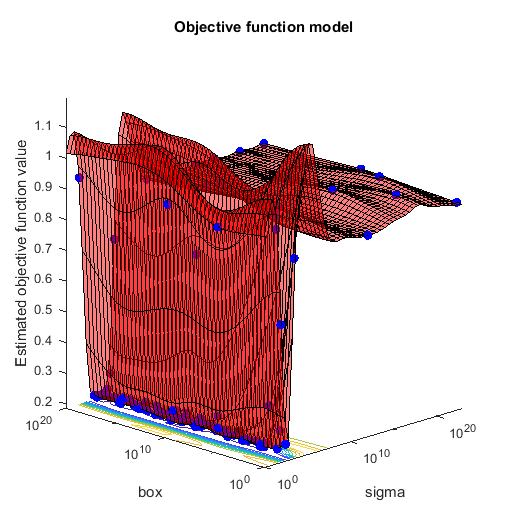
\includegraphics[width=0.5\textwidth]{Chapter4/Figs/MaskedOptimIteration2.png}
	\caption{HOG cells, blocs and overlapping}
	\label{fig:opt1}
\end{figure}

%%%%%%%

%%%%%%%%%%%%%%%%%%%%%%%%eLFW%%%DVM%%%%%%%%%%%%%%%%%%%%%%%%%%%%%%%%%%%%%%
\begin{table}[tb]
	\fontsize{12}{12}
	\centering
	\textbf{
		\caption{Confusion matrix for SVM classification of the eLFW database with the importance mask shown in Figure \ref{fig:impportSteps} }\label{eLFW&SVM}}
	
	
	\begin{tabular}{@{}|l|c|c|c|c|c|c|c|@{}}
		\hline
		& \textbf{FE}    & \textbf{AN}    & \textbf{DI}    & \textbf{HA} & \textbf{NE} & \textbf{SA}    & \textbf{SU}    \\ \hline
		\textbf{FE} & \textbf{0.237} & 0.137          & 0.184             & 0.042           & 0.058       & 0.153           & 0.189          \\ \hline
		\textbf{AN} & 0.058              & \textbf{0.733} & 0.025          & 0.000           & 0.008          & 0.075          & 0.100 \\ \hline
		\textbf{DI} & 0.056              & 0.025              & \textbf{0.750} & 0.025           & 0.038           & 0.025          & 0.081              \\ \hline
		\textbf{HA} & 0.018              & 0.021              & 0.15              & \textbf{0.845}  & 0.033          & 0.018              & 0.048              \\ \hline
		\textbf{NE} & 0.025              & 0.013              & 0.038              & 0.063           & \textbf{0.829}  & 0.021 & 0.013              \\ \hline
		\textbf{SA} & 0.175          & 0.125          & 0.060          & 0.010          & 0.025           & \textbf{0.495} & 0.110              \\ \hline
		\textbf{SU} & 0.157               & 0.114              & 0.143               & 0.029         & 0.000       & 0.014              & \textbf{0.543} \\ \hline
	\end{tabular}
\end{table}
%%%%%%%%%%%%%%%%%%%%%%%%%%%%%%%%%%%%%%%%%%%%%%%%%%%%%%%%%%%%%%%%%
Table \ref{KDEFSVM} illustrates the same KDEF photos with Support Vector Machine classification (SVM) for whole facial features without applying the importance mask. To optimise the SVM, we need to find the best SVM parameters, Kernel coefficient $ \gamma$ and  $C$. We used Bayesian optimization method which is a powerful method to optimise functions \citep{mockus2012bayesian}. The main idea of our optimisation is to minimise the cross-validation loss, by finding the best SVM parameters $ \gamma$ and  $C$. The best parameters were where $\sigma = 6423.7$, and $ C  = 1.2333e+19$. 
By comparing the outcome presented in table \ref{KDEFSVM} with that shown in \ref{table:RF_KDEF_compined}, the random forest gave slightly better outcomes. The SVM overall classification rate is $72\%$. %0.789.
After applying the KDEF mask, The SVM overall classification rate rose to $81\%$ as shown in table \ref{MASKEDKDEFSVM}. SVM was optimised and its parameters were $\sigma = 43482$, and $ C  = 9.2891e+18$. 

Table \ref{eLFW&SVM} illustrates a confusion matrix of testing the important features by SVM. Compared to the results in the right table \ref{Table:eLFW&Random}, random forest still gives better results that SVM with the important combined features. According to table \ref{eLFW&SVM}, the overall classification is $66.3\%$ where the overall classification in the table \ref{Table:eLFW&Random} was $67.3\%$.

\begin{equation}
\label{eq:CrossVal}
CVA =  \sum_{i=1}^{K} \frac{A_i}{k}
\end{equation}\tabularnewline



where $k =$ number of folds used, and $Ai =$ accuracy measure of each fold.



%%%%%%%%%%%%%%%%%%%%%%%%%%%%%%%%%%%%%%%%%%%%%%%%%%%%%%%%%%%%%%%%%
\begin{table}[tb]
	\fontsize{12}{12}
	\centering
	\textbf{
		\caption{Confusion matrix for SVM classification of the KDEF database without the importance mask. The overall accuracy is \%72
		} \label{KDEFSVM}} 
	
	\begin{tabular}{@{}|l|c|c|c|c|c|c|c|@{}}    \hline
		& \textbf{FE}     & \textbf{AN}    & \textbf{DI}    & \textbf{HA} & \textbf{NE} & \textbf{SA}    & \textbf{SU}   \\ \hline
		\textbf{FE} & \textbf{0.643} & 0.014          & 0.057          & 0.100           & 0.029           & 0.071          & 0.086 \\ \hline
		\textbf{AN} & 0.043          & \textbf{0.671} & 0.071          & 0.000           & 0.043           & 0.086          & 0.086 \\ \hline
		\textbf{DI} & 0.086          & 0.057          & \textbf{0.714} & 0.000           & 0.000           & 0.071          & 0.071  \\ \hline
		\textbf{HA} & 0.000          & 0.000          & 0.000          & \textbf{0.900}  & 0.057           & 0.014          & 0.029  \\ \hline
		\textbf{NE} & 0.000          & 0.000           & 0.014          & 0.071           & \textbf{0.843}  & 0.057           & 0.014 \\ \hline
		\textbf{SA} & 0.068          & 0.043          & 0.071          & 0.000           & 0.029           & \textbf{0.657}  & 0.114   \\ \hline
		\textbf{SU} & 0.157          & 0.057          & 0.043          & 0.014           & 0.014           & 0.071           & \textbf{0.643} \\ \hline
	\end{tabular}
\end{table}
%%%%%%%%%%%%%%%%%%%%%%%%%%%%%%%%%%%%%%%%%%%%%%%%%%%%%%%%%%%%%%%%%

%%%%%%%%%%%%%%%%%%%%%%%%%%%%%%%%%%%%%%%%%%%%%%%%%%%%%%%%%%%%%%%%%
\begin{table}[H]
	\fontsize{12}{12}
	\centering
	\textbf{
		\caption{Confusion matrix for SVM classification of the KDEF database with the importance mask shown in figure \ref{fig:impportSteps}. The ovrall accuracy is $81 \%$.} \label{MASKEDKDEFSVM}} 
	
	\begin{tabular}{@{}|l|c|c|c|c|c|c|c|@{}}  \hline
		& \textbf{FE}     & \textbf{AN}    & \textbf{DI}    & \textbf{HA} & \textbf{NE} & \textbf{SA}    & \textbf{SU} \\ \hline
		\textbf{FE} & \textbf{0.714} & 0.057          & 0.043          & 0.000           & 0.000            & 0.100          & 0.086 \\ \hline
		\textbf{AN} & 0.043          & \textbf{0.686} & 0.071          & 0.000           & 0.029           & 0.086           & 0.086 \\ \hline
		\textbf{DI} & 0.043          & 0.057          & \textbf{0.786} & 0.000           & 0.000           & 0.057           & 0.057 \\ \hline
		\textbf{HA} & 0.000          & 0.000          & 0.000          & \textbf{0.957}  & 0.029           & 0.000           & 0.014 \\ \hline
		\textbf{NE} & 0.000          & 0.000           & 0.000          & 0.057           & \textbf{0.900}  & 0.029           & 0.014\\ \hline
		\textbf{SA} & 0.057          & 0.057          & 0.043          & 0.000           & 0.000           & \textbf{0.771}  & 0.071 \\ \hline
		\textbf{SU} & 0.071          & 0.029          & 0.014          & 0.014           & 0.000           & 0.029           & \textbf{0.843} \\ \hline
	\end{tabular}
\end{table}
%%%%%%%%%%%%%%%%%%%%%%%%%%%%%%%%%%%%%%%%%%%%%%%%%%%%%%%%%%%%%%%%%











%\begin{figure}[H]
%  \centering
%      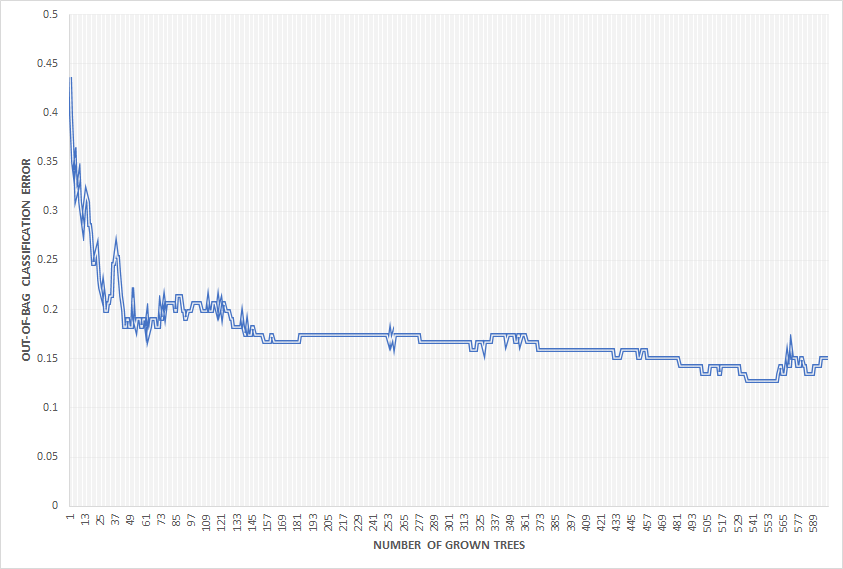
\includegraphics[width=1\textwidth]{Chapter4/Figs/fearvassup.png}
%  \caption{The out-of-bag error for 2-Class Random forest (Fear vs Surprise) - Accuracy is: 0.873      \label{fig:newLayer}}
%\end{figure}


%\begin{table}[H]
%\centering
%\caption{Example 1: A fear image with wrong classification decision}
%\label{Table:wrongClassImage}
%\begin{tabular}{|l|c|c|c|c|c|c|c|c|}
%\hline
%                  & \textbf{Fear} & \textbf{Anger} & \textbf{Disgust} & \textbf{Happy} & \textbf{Neutral} & \textbf{Sad} & \textbf{Surprise} & \textbf{Total} \\ \hline
%\textbf{Fear}     & x             & 0.87           & 0.88             & 0.85           & 0.49             & 0.62         & 0.38              & \textbf{4.10}  \\ \hline
%\textbf{Anger}    & 0.13          & x              & 0.80             & 0.73           & 0.12             & 0.22         & 0.12              & \textbf{2.11}  \\ \hline
%\textbf{Disgust}  & 0.12          & 0.21           & x                & 0.56           & 0.08             & 0.10         & 0.07              & \textbf{1.13}  \\ \hline
%\textbf{Happy}    & 0.15          & 0.27           & 0.44             & x              & 0.07             & 0.11         & 0.08              & \textbf{1.12}  \\ \hline
%\textbf{Neutral}  & 0.51          & 0.88           & 0.92             & 0.93           & x                & 0.64         & 0.48              & \textbf{4.36}  \\ \hline
%\textbf{Sad}      & 0.38          & 0.78           & 0.90             & 0.89           & 0.36             & x            & 0.31              & \textbf{3.63}  \\ \hline
%\textbf{Surprise} & 0.62          & 0.88           & 0.93             & 0.92           & 0.51             & 0.69         & x                 & \textbf{4.55}  \\ \hline
%\end{tabular}
%\end{table}
%
%
%
%
%
%
%
%\begin{table}[H]
%\centering
%\caption{Example 3: A fear image with correct classification decision}
%\label{Table:CorrectClassImage}
%\begin{tabular}{|l|c|c|c|c|c|c|c|c|}
%\hline
%                  & \textbf{Fear} & \textbf{Anger} & \textbf{Disgust} & \textbf{Happy} & \textbf{Neutral} & \textbf{Sad} & \textbf{Surprise} & \textbf{Total} \\ \hline
%\textbf{Fear}     & x             & 0.94           & 0.93             & 0.86           & 0.85             & 0.69         & 0.48              & \textbf{4.76}  \\ \hline
%\textbf{Anger}    & 0.06          & x              & 0.78             & 0.77           & 0.27             & 0.16         & 0.10              & \textbf{2.13}  \\ \hline
%\textbf{Disgust}  & 0.07          & 0.23           & x                & 0.57           & 0.16             & 0.12         & 0.12              & \textbf{1.27}  \\ \hline
%\textbf{Happy}    & 0.14          & 0.23           & 0.43             & x              & 0.18             & 0.28         & 0.13              & \textbf{1.40}  \\ \hline
%\textbf{Neutral}  & 0.15          & 0.73           & 0.84             & 0.81           & x                & 0.19         & 0.31              & \textbf{3.04}  \\ \hline
%\textbf{Sad}      & 0.31          & 0.84           & 0.88             & 0.72           & 0.81             & x            & 0.31              & \textbf{3.86}  \\ \hline
%\textbf{Surprise} & 0.52          & 0.90           & 0.88             & 0.86           & 0.69             & 0.70         & x                 & \textbf{4.54}  \\ \hline
%\end{tabular}
%\end{table}
%
%
%
%



\section{Weighted pairwise classification}
\label{sec:weight-pairw-class}



Random forest classifiers combine decision trees which are naturally capable of multi-class classification, as opposed to dichotomous classifiers, such as SVMs, for which strategies such as one-versus-all or pairwise voting must be employed.
%%%%%%%%%%%%%%%%%%%%%%%%%%%%%%%%%%%%%%%%%%%%%%%%%%%%%%%%%%%%%%%%%
\begin{table}[tb]
	\caption[caption]{Posterior probabilities for two different fear images tested by the 21 random classifiers, the left has been wrongly classified and the right correctly classified.}
	\label{tab:Correct&Wrongclassification}
	\begin{minipage}{.5\linewidth}
		\centering
		Wrong classification decision\\[1mm]
		\resizebox{.95\textwidth}{!}{%
			\begin{tabular}{|l|c|c|c|c|c|c|c|c|}
				
				\hline
				& \textbf{Fear} & \textbf{Anger} & \textbf{Disgust} & \textbf{Happy} & \textbf{Neutral} & \textbf{Sad} & \textbf{Surprise} & \textbf{Total} \\ \hline
				\textbf{Fear}     & x             & 0.87           & 0.88             & 0.85           & 0.49             & 0.62         & 0.38              & \textbf{4.10}  \\ \hline
				\textbf{Anger}    & 0.13          & x              & 0.80             & 0.73           & 0.12             & 0.22         & 0.12              & \textbf{2.11}  \\ \hline
				\textbf{Disgust}  & 0.12          & 0.21           & x                & 0.56           & 0.08             & 0.10         & 0.07              & \textbf{1.13}  \\ \hline
				\textbf{Happy}    & 0.15          & 0.27           & 0.44             & x              & 0.07             & 0.11         & 0.08              & \textbf{1.12}  \\ \hline
				\textbf{Neutral}  & 0.51          & 0.88           & 0.92             & 0.93           & x                & 0.64         & 0.48              & \textbf{4.36}  \\ \hline
				\textbf{Sad}      & 0.38          & 0.78           & 0.90             & 0.89           & 0.36             & x            & 0.31              & \textbf{3.63}  \\ \hline
				\textbf{Surprise} & 0.62          & 0.88           & 0.93             & 0.92           & 0.51             & 0.69         & x                 & \textbf{4.55}  \\ \hline
		\end{tabular}}
		
	\end{minipage}\hfill
	\begin{minipage}{.5\linewidth}
		\centering
		Correct classification decision\\[1mm]
		\resizebox{.95\textwidth}{!}{%
			\begin{tabular}{|l|c|c|c|c|c|c|c|c|}
				\hline
				& \textbf{Fear} & \textbf{Anger} & \textbf{Disgust} & \textbf{Happy} & \textbf{Neutral} & \textbf{Sad} & \textbf{Surprise} & \textbf{Total} \\ \hline
				\textbf{Fear}     & x             & 0.94           & 0.93             & 0.86           & 0.85             & 0.69         & 0.48              & \textbf{4.76}  \\ \hline
				\textbf{Anger}    & 0.06          & x              & 0.78             & 0.77           & 0.27             & 0.16         & 0.10              & \textbf{2.13}  \\ \hline
				\textbf{Disgust}  & 0.07          & 0.23           & x                & 0.57           & 0.16             & 0.12         & 0.12              & \textbf{1.27}  \\ \hline
				\textbf{Happy}    & 0.14          & 0.23           & 0.43             & x              & 0.18             & 0.28         & 0.13              & \textbf{1.40}  \\ \hline
				\textbf{Neutral}  & 0.15          & 0.73           & 0.84             & 0.81           & x                & 0.19         & 0.31              & \textbf{3.04}  \\ \hline
				\textbf{Sad}      & 0.31          & 0.84           & 0.88             & 0.72           & 0.81             & x            & 0.31              & \textbf{3.86}  \\ \hline
				\textbf{Surprise} & 0.52          & 0.90           & 0.88             & 0.86           & 0.69             & 0.70         & x                 & \textbf{4.54}  \\ \hline
		\end{tabular}}
		
	\end{minipage} 
\end{table}
In an effort to reduce the misclassifications of fear, anger, disgust and surprise, we also investigated the use of pairwise classifiers for classifying emotions.  In this framework, a single classifier is trained to discriminate between a pair of classes. The item is then assigned to the class which receives the majority of votes from the pairwise classifiers. 

For n-Class pairwise classification, the number of the classifiers is $c=\frac{n(n-1)}{2}$, so to classify the $n=7$ emotions, there are 21 pairs of classifiers.  Each pair of facial expressions class was used to train one random forest classifier. At the testing stage, each image was tested with all the 21 classifiers. For each facial expression, we calculate all votes from each classifier to get the total vote. The maximum vote for the seven expressions is the final decision.  

As example, table \ref{tab:Correct&Wrongclassification} shows the posterior probabilities (see equation \ref{eq:maximum_posteriori}) of 21 random forest classifiers for two different images whose correct class was fear. Each cell in the tables is the posterior probability (classifier score) with the expression in the same row vs the expression in the same column. In the left table, the image has been wrongly classified as surprise (maximum total 4.55). Table \ref{tab:Correct&Wrongclassification} (right) shows another fear image which has been correctly classified (maximum total 4.76).



Table \ref{table:PRF_vs_PSVM} shows the accuracy of RF and SVM classifiers on the KDEF data, using the usual 10-fold cross-validation. We noticed that both classifier's performance are very similar, and there is no significant difference between overall scores; while the RF's average accuracy was 0.963 and SVMs was 0.962. There is one advantage of SVMs:  all of the 21 classifiers gave an accuracy of over 90\%, whereas RF gave two results lower than 90\% with fear vs surprise, and neutral vs sad. 
% Figures \ref{fig:Happy_Surprise_OOB} and \ref{fig:Happy_Fear_OOB} show the OOB error while trees building.


%%%%%%%%%%%%%%%%%%%%%%%%%%%%%%%%%%%%%%%%%%%%%%%%%%%%%%%%%%%%%%%%%%
\begin{table}[tb]
	\fontsize{12}{12}
	\centering
	\caption{Pairwise RF classifiers and pairwise SVM classifiers performance with KDEF.}
	\label{table:PRF_vs_PSVM}
	\resizebox{.8\textwidth}{!}{%
		
		\begin{tabular}{|l|c|c|l|c|c|}
			\hline
			\textbf{Classifier} & \multicolumn{1}{l|}{\textbf{RF}} & \multicolumn{1}{l|}{\textbf{SVM}} & \textbf{Classifier} & \multicolumn{1}{l|}{\textbf{RF}} & \multicolumn{1}{l|}{\textbf{SVM}} \\ \hline
			Fear vs Anger       & 0.956  & 0.935         & Disgust vs Happy        & 0.976  & 0.978        \\ \hline
			Fear vs Disgust     & 0.968  & 0.978         & Disgust vs Neutral      & 0.999  & 0.993        \\ \hline
			Fear vs Happy       & 0.976  & 0.978         & Disgust vs Sad          & 0.960  & 0.942        \\ \hline
			Fear vs Neutral     & 0.940  & 0.957         & Disgust vs Surprise     & 0.988  & 1.000        \\ \hline
			Fear vs Sad         & 0.920  & 0.900         & Happy vs Neutral        & 0.999  & 0.993        \\ \hline
			Fear vs Surprise    & 0.883  & 0.900         & Happy vs Sad            & 0.987  & 0.971        \\ \hline
			Anger vs Disgust    & 0.935  & 0.900         & Happy vs Surprise       & 0.999  & 0.993        \\ \hline
			Anger vs Happy      & 0.993  & 0.985         & Neutral vs Sad          & 0.895  & 0.940        \\ \hline
			Anger vs Neutral    & 0.952  & 0.950         & Neutral vs Surprise     & 0.984  & 0.985        \\ \hline
			Anger vs Sad        & 0.936  & 0.950         & Sad vs Surprise         & 0.976  & 0.978        \\ \hline
			Anger vs Surprise   & 0.994  & 1.000        & \multicolumn{1}{c|}{\textbf{Overall}} & \textbf{0.963} & \textbf{0.962}\\ \hline
	\end{tabular}}
\end{table}
%%%%%%%%%%%%%%%%%%%%%%%%%%%%%%%%%%%%%%%%%%%%%%%%%%%%%%%%%%%%%%%%%%

Table \ref{NewConfusion} shows the RF pairwise classification results of the KDEF data, by comparing these results with the results in table  \ref{table:RF_KDEF_compined}, it is clear that pairwise classification has enhanced the overall accuracy from 89\% to be  92\%. We notice that the fear expression classification rate has significantly been improved. Table \ref{table:us-vs-others} demonstrates that when evaluated on the KDEF data our proposed method using random forest classifiers and masked LBP, HOG and D-SURF features compares favourably with another state of the art techniques.  


%%%%%%%%%%%%%%%%%%%%%%%%%%%%%%%%%%%%%%%%%%%%%%%%%%%%%%%%%%%%%%%%%%
\begin{table}[tb]
	\fontsize{12}{12}
	
	\centering
	\textbf{
		\caption{Random Forestrs pair-classifiers optimised weights}\label{table:optimised_weights}} 
	\selectfont
	%  \resizebox{1\textwidth}{!}{%
	\begin{tabular}{@{}|l|c|c|c|c|c|c|c|c|@{}}
		\hline
		& \textbf{Fear} & \textbf{Anger} & \textbf{Disgust} & \textbf{Happy} & \textbf{Neutral} & \textbf{Sad} & \textbf{Surprise}  \\ \hline
		\textbf{Fear}     & x             & 0.198       & 0.202         & 0.159       & 0.106         & 0.159     & 0.176            \\ \hline
		\textbf{Anger}    & 0.226      & x              & 0.247         & 0.232       & 0.450         & 0.127     & 0.122          \\ \hline
		\textbf{Disgust}  & 0.205      & 0.187       & x                & 0.175       & 0.114         & 0.155     & 0.164           \\ \hline
		\textbf{Happy}    & 0.210      & 0.187        & 0.184         & x              & 0.114         & 0.150      & 0.156 \\ \hline
		\textbf{Neutral}  & 0.216      & 0.187       & 0.174         & 0.107       & x                & 0.157     & 0.159           \\ \hline
		\textbf{Sad}      & 0.206      & 0.195       & 0.172          & 0.106       & 0.158         & x            & 0.164          \\ \hline
		\textbf{Surprise} & 0.204      & 0.190       & 0.171         & 0.116       & 0.151         & 0.169     & x              \\ \hline 
	\end{tabular}%}
\end{table}
%%%%%%%%%%%%%%%%%%%%%%%%%%%%%%%%%%%%%%%%%%%%%%%%%%%%%%%%%%%%%%%%%%

In most pairwise architectures each of the constituent classifiers has an equal vote.  Here we weigh the votes from each classifier and learn appropriate weights by optimising the classification accuracy of a validation set. 
More specifically, suppose $y_{ij}(\bx_n) \in [0, 1]$ is the output of the classifier
discriminating between classes $i$ and $j$ for image features $\bx_n$.  Here we use  random forests for each dichotomous classifier, so that $y_{ij}(\bx_n)$ is the proportion of decision trees in the $(i,j)$-th forest that voted for class $i$. Then the overall score for
class $i$ is
\begin{equation}
Y_i(\bx_n) = \sum_{j\ne i} \lambda_{ij} y_{ij}(\bx_n)
\end{equation}
where the weights are $\lambda_{ij}$, and the image is assigned  to the
class with the largest overall score: $\argmax_i Y_i(\bx_n)$. The weights are constrained to be non-negative, $\lambda_{ij} \ge 0 $ for all $i$ and $j$,  and
we demand that $\sum_{j} \lambda_{ij} = 1 $ for all $i$. 

Training takes place in two phases.  First, the constituent classifiers are independently trained on the pairs of classes.  Secondly, the accuracy of the overall classifier on a second training data set is maximised by optimising the voting weights using an evolutionary optimiser.  Here we used CMA-ES \citep{hansen2006eda}, a popular and effective evolutionary optimiser.  Constraints were enforced by working in terms of variables $\theta_{ij}$ with
\begin{equation}
\lambda_{ij} = \frac{\theta_{ij} }{ \sum_{k}
	\theta_{ik}}.
\end{equation}
We note that the procedure is efficient because once the pairwise classifiers have been trained, classification scores $y_{ij}(\bx_n)$ need only be calculated once before optimisation of the weights.

%%%%%%%%%%%%%%%%%%%%%%%%%%%%%%%%%%%%%%%%%%%%%%%%%%%%%%%%%%%%%%%%%%
\begin{table}[tb]
	\fontsize{12}{12}
	
	\centering
	\caption{Confusion matrix for equally weighted pairwise classification on the KDEF data.  
		Overall accuracy is 92\%.}
	\label{NewConfusion}
	\begin{tabular}{@{}|l|c|c|c|c|c|c|c|@{}}  \hline
		& \textbf{FE}     & \textbf{AN}    & \textbf{DI}    & \textbf{HA} & \textbf{NE} & \textbf{SA}    & \textbf{SU} \\ \hline
		\textbf{FE}          & \textbf{0.814} & 0.029          & 0.043            & 0.000          & 0.000            & 0.029          & 0.086             \\ \hline
		\textbf{AN}         & 0.000          & \textbf{0.886} & 0.043            & 0.000          & 0.000            & 0.071          & 0.000             \\ \hline
		\textbf{DI}       & 0.000          & 0.043          & \textbf{0.929}   & 0.000          & 0.000            & 0.029          & 0.000             \\ \hline
		\textbf{HA}         & 0.000          & 0.000          & 0.000            & \textbf{0.986} & 0.014            & 0.000          & 0.000             \\ \hline
		\textbf{NE}       & 0.000          & 0.000          & 0.000            & 0.014          & \textbf{0.986}   & 0.000          & 0.000             \\ \hline
		\textbf{Sad}           & 0.029          & 0.029          & 0.043            & 0.000          & 0.000            & \textbf{0.900} & 0.000             \\ \hline
		\textbf{SU}      & 0.029          & 0.000          & 0.014            & 0.000          & 0.000            & 0.000          & \textbf{0.957}    \\ \hline
	\end{tabular}
\end{table}
%%%%%%%%%%%%%%%%%%%%%%%%%%%%%%%%%%%%%%%%%%%%%%%%%%%%%%%%%%%%%%%%%%
Table \ref{table:optimised_weights} shows the weights  $\lambda_{ij}$ obtained by the optimisation processes.
Table \ref{tab:KDEF+eLFW-pairwise} shows the confusion matrix obtained with the optimised pairwise classification using 10-fold cross-validation testing.  The accuracies for the data sets have increased to $95.1\%$ for KDEF and $76.6\%$ for eLFW. As can be seen from the confusion matrix, classification accuracies of fear, anger, surprise and disgust have increased substantially, although for the eLFW data there is still considerable misclassification of fear (confused with disgust and surprise), sadness (confused with fear and anger) and surprise (confused with neutral, fear, anger and disgust). We remark that these emotions are all often expressed through a grimacing expression which may account for the difficulty in distinguishing them. Furthermore, these are the emotions about which the citizens showed the most disagreement (see section\ref{sec:Comparison_citizen}). 





%\begin{table}[tb]
%\centering
%\caption{Example 1: A fear image with wrong classification decision}
%\label{Table:wrongClassImage}
%\begin{tabular}{|l|c|c|c|c|c|c|c|c|}
%\hline
%                  & \textbf{Fear} & \textbf{Anger} & \textbf{Disgust} & \textbf{Happy} & \textbf{Neutral} & \textbf{Sad} & \textbf{Surprise} & \textbf{Total} \\ \hline
%\textbf{Fear}     & x             & 0.87           & 0.88             & 0.85           & 0.49             & 0.62         & 0.38              & \textbf{4.10}  \\ \hline
%\textbf{Anger}    & 0.13          & x              & 0.80             & 0.73           & 0.12             & 0.22         & 0.12              & \textbf{2.11}  \\ \hline
%\textbf{Disgust}  & 0.12          & 0.21           & x                & 0.56           & 0.08             & 0.10         & 0.07              & \textbf{1.13}  \\ \hline
%\textbf{Happy}    & 0.15          & 0.27           & 0.44             & x              & 0.07             & 0.11         & 0.08              & \textbf{1.12}  \\ \hline
%\textbf{Neutral}  & 0.51          & 0.88           & 0.92             & 0.93           & x                & 0.64         & 0.48              & \textbf{4.36}  \\ \hline
%\textbf{Sad}      & 0.38          & 0.78           & 0.90             & 0.89           & 0.36             & x            & 0.31              & \textbf{3.63}  \\ \hline
%\textbf{Surprise} & 0.62          & 0.88           & 0.93             & 0.92           & 0.51             & 0.69         & x                 & \textbf{4.55}  \\ \hline
%\end{tabular}
%\end{table}
%
%
%
%\begin{table}[tb]
%\centering
%\caption{Example 3: A fear image with correct classification decision}
%\label{Table:CorrectClassImage}
%\begin{tabular}{|l|c|c|c|c|c|c|c|c|}
%\hline
%                  & \textbf{Fear} & \textbf{Anger} & \textbf{Disgust} & \textbf{Happy} & \textbf{Neutral} & \textbf{Sad} & \textbf{Surprise} & \textbf{Total} \\ \hline
%\textbf{Fear}     & x             & 0.94           & 0.93             & 0.86           & 0.85             & 0.69         & 0.48              & \textbf{4.76}  \\ \hline
%\textbf{Anger}    & 0.06          & x              & 0.78             & 0.77           & 0.27             & 0.16         & 0.10              & \textbf{2.13}  \\ \hline
%\textbf{Disgust}  & 0.07          & 0.23           & x                & 0.57           & 0.16             & 0.12         & 0.12              & \textbf{1.27}  \\ \hline
%\textbf{Happy}    & 0.14          & 0.23           & 0.43             & x              & 0.18             & 0.28         & 0.13              & \textbf{1.40}  \\ \hline
%\textbf{Neutral}  & 0.15          & 0.73           & 0.84             & 0.81           & x                & 0.19         & 0.31              & \textbf{3.04}  \\ \hline
%\textbf{Sad}      & 0.31          & 0.84           & 0.88             & 0.72           & 0.81             & x            & 0.31              & \textbf{3.86}  \\ \hline
%\textbf{Surprise} & 0.52          & 0.90           & 0.88             & 0.86           & 0.69             & 0.70         & x                 & \textbf{4.54}  \\ \hline
%\end{tabular}
%\end{table}









%\begin{figure}
%\centering
%\begin{subfigure}{.5\textwidth}
%  \centering
%  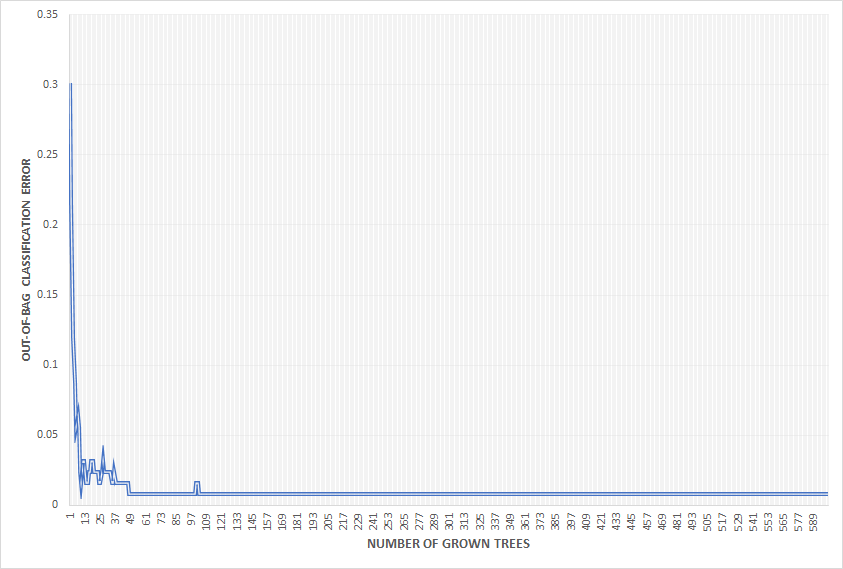
\includegraphics[width=1\linewidth]{Chapter4/Figs/hapvssub.png}
%  \caption{(Happy vs Surprise)  Accuracy is: 0.993 }
%  \label{fig:Happy_Surprise_OOB}
%\end{subfigure}%
%\begin{subfigure}{.5\textwidth}
%  \centering
%  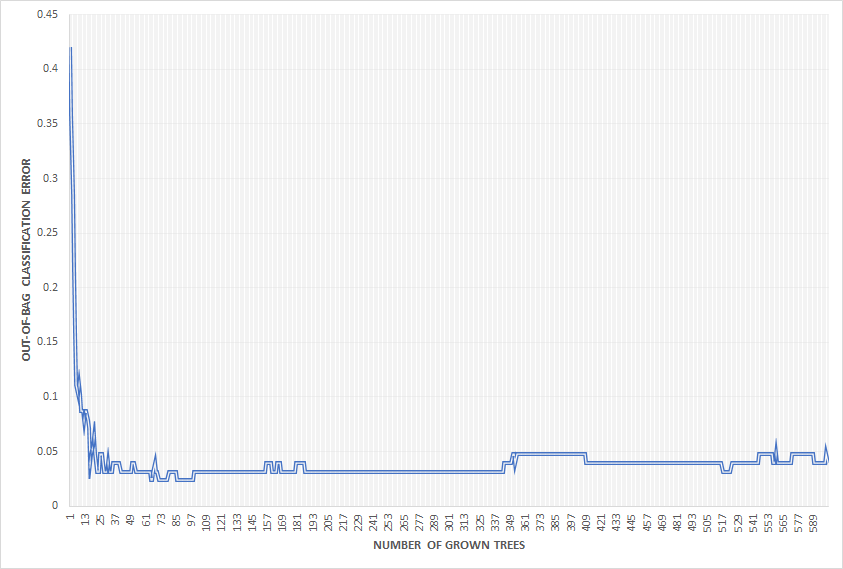
\includegraphics[width=1\linewidth]{Chapter4/Figs/hapvsfear.png}
%  \caption{(Happy vs Fear) - Accuracy is: 0.976 }
%  \label{fig:Happy_Fear_OOB}
%\end{subfigure}
%\caption{The out-of-bag error for 2-Class Random forest}
%\label{fig:test}
%\end{figure}


%
%
%\begin{figure}[H]
%  \centering
%      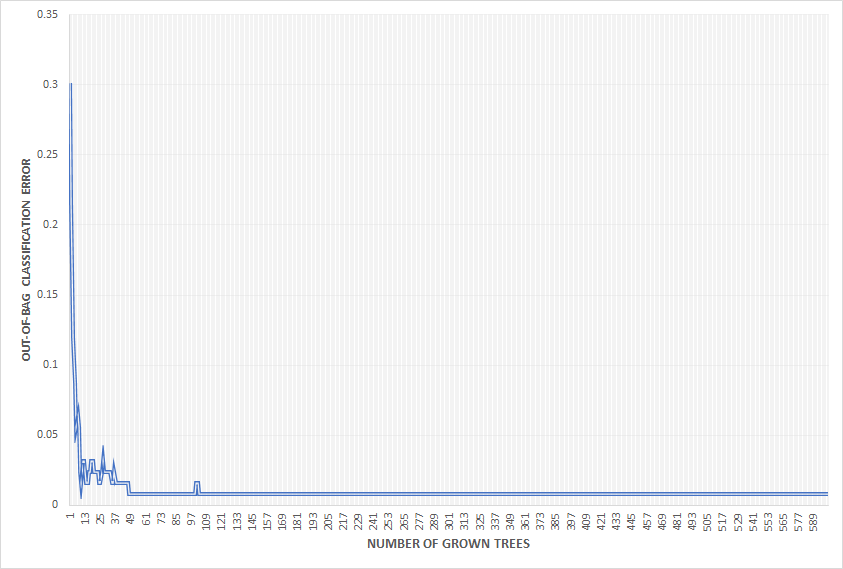
\includegraphics[width=.5\textwidth]{Chapter4/Figs/hapvssub.png}
%  \caption{The out-of-bag error for 2-Class Random forest (Happy vs Surprise)  Accuracy is: 0.993       \label{fig:Happy_Surprise_OOB}}
%\end{figure}
%
%
%\begin{figure}[H]
%  \centering
%      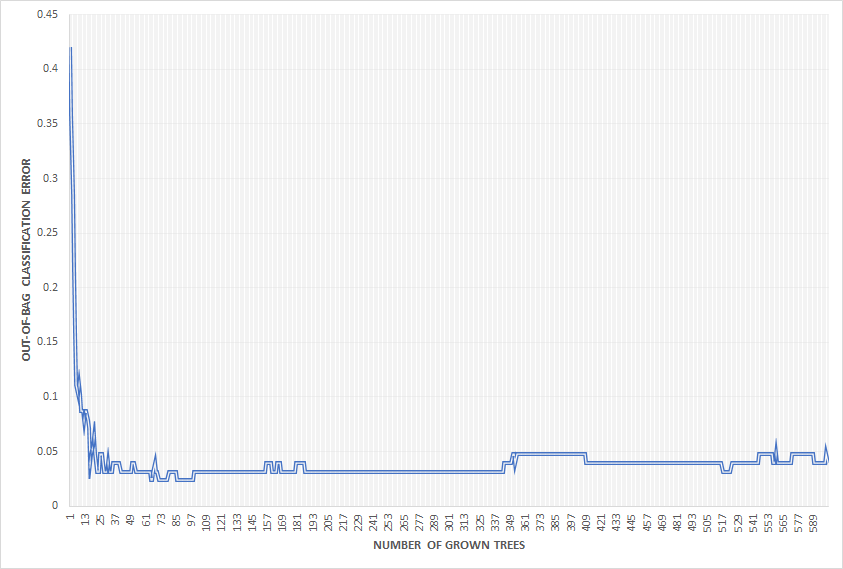
\includegraphics[width=.5\textwidth]{Chapter4/Figs/hapvsfear.png}
%  \caption{The out-of-bag error for 2-Class Random forest (Happy vs Fear) - Accuracy is: 0.976     \label{fig:Happy_Fear_OOB}}
%\end{figure}








%%%%%%%%%%%%%%%%%%%%%%%%%%%%%%%%%%%%%%%%%%%%%%%%%%%%%%%%%%%%%%%%%%
\begin{table}[tb]
	\caption[caption]{Confusion matrices weighted pairwise classification of the KDEF and eLFW databases. The overall accuracy is $95.1\%$ for KDEF and $76.6\%$ for eLFW}
	\label{tab:KDEF+eLFW-pairwise}
	\begin{minipage}{.5\linewidth}
		\centering
		KDEF\\[1mm]
		\resizebox{.97\textwidth}{!}{%
			\begin{tabular}{@{}|l|c|c|c|c|c|c|c|@{}}
				\toprule
				\multicolumn{1}{|c|}{} & \textbf{FE}  & \textbf{AN} & \textbf{DI} & \textbf{HA} & \textbf{NE} & \textbf{SA}   & \textbf{SU} \tabularnewline \midrule
				\textbf{FE}      & \textbf{0.914} & 0.029           & 0.000            & 0.000         & 0.000   & 0.000     & 0.057   \tabularnewline \midrule
				\textbf{AN}      & 0.000          & \textbf{0.943} & 0.014            & 0.000          & 0.000            & 0.043          & 0.000  \tabularnewline \midrule
				\textbf{DI}      & 0.000          & 0.014          & \textbf{0.971}   & 0.000          & 0.000            & 0.014          & 0.000  \tabularnewline \midrule
				\textbf{HA}      & 0.000          & 0.000          & 0.000            & \textbf{0.986} & 0.014            & 0.000          & 0.000  \tabularnewline \midrule
				\textbf{NE}      & 0.000          & 0.000          & 0.000            & 0.014          & \textbf{0.986}   & 0.000          & 0.000   \tabularnewline \midrule
				\textbf{SA}      & 0.043          & 0.029          & 0.043            & 0.000          & 0.000            & \textbf{0.886} & 0.000    \tabularnewline \midrule
				\textbf{SU}      & 0.014          & 0.000          & 0.014            & 0.000          & 0.000            & 0.000          & \textbf{0.971} \tabularnewline \bottomrule
		\end{tabular}}
		
	\end{minipage}\hfill
	\begin{minipage}{.5\linewidth}
		\centering
		eLFW\\[1mm]
		\resizebox{.97\textwidth}{!}{%
			\begin{tabular}{@{}|l|c|c|c|c|c|c|c|@{}}
				\toprule
				& \textbf{FE}     & \textbf{AN}       & \textbf{DI}      & \textbf{HA} & \textbf{NE} & \textbf{SA}    & \textbf{SU}      \tabularnewline \midrule
				\textbf{FE} & \textbf{0.495}  & 0.089             & 0.142   & 0.011            & 0.042             & 0.074                 & 0.147   \tabularnewline \midrule
				\textbf{AN} & 0.025           & \textbf{0.792}    & 0.050            & 0.000             & 0.000           & 0.083          & 0.050  \tabularnewline \midrule
				\textbf{DI} & 0.056           & 0.019             & \textbf{0.788}   & 0.044             & 0.031           & 0.025          & 0.038   \tabularnewline \midrule
				\textbf{HA} & 0.003           & 0.012             & 0.003            & \textbf{0.970}   & 0.009            & 0.003          & 0.000   \tabularnewline \midrule
				\textbf{NE} & 0.004           & 0.013             & 0.000            & 0.017             & \textbf{0.938}  & 0.029          & 0.000  \tabularnewline \midrule
				\textbf{SA} & 0.150           & 0.130             & 0.065            & 0.010             & 0.010          & \textbf{0.535} & 0.100   \tabularnewline \midrule
				\textbf{SU} & 0.086           & 0.086             & 0.071            & 0.014             & 0.129           & 0.086          & \textbf{0.529} \tabularnewline \bottomrule
		\end{tabular}}
		
	\end{minipage} 
\end{table}
%%%%%%%%%%%%%%%%%%%%%%%%%%%%%%%%%%%%%%%%%%%%%%%%%%%%%%%%%%%%%%%%%%

%\begin{figure}[tb]
%  \centering
%      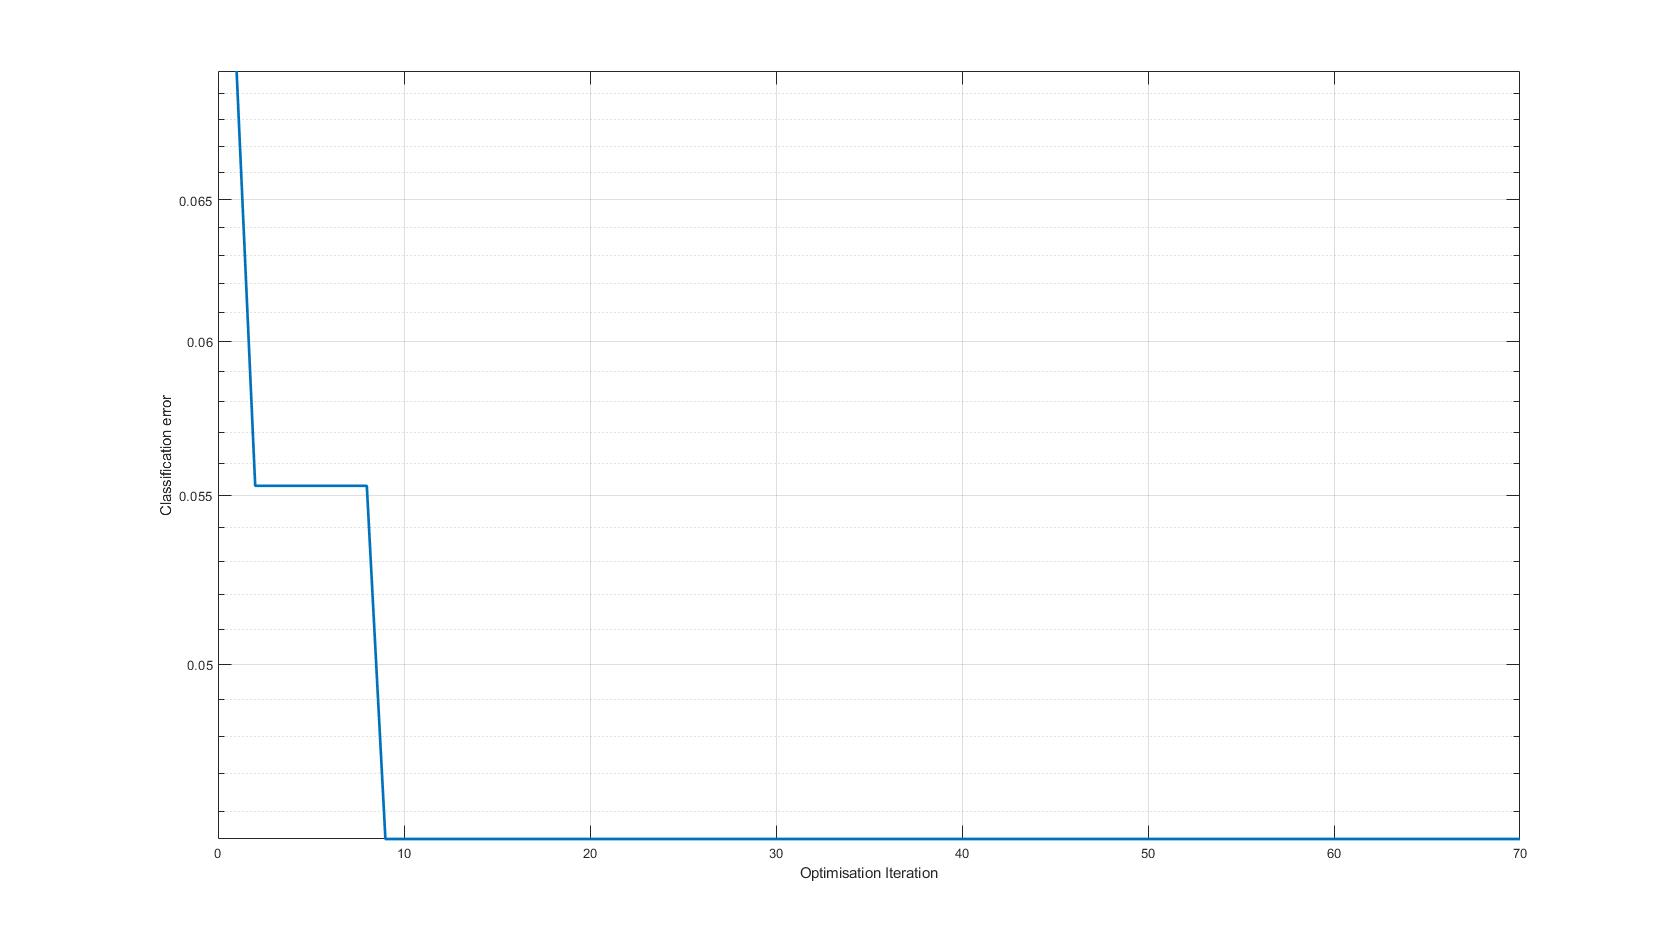
\includegraphics[width=1\textwidth]{Chapter4/Figs/Optimisition.jpg}
%  \caption{Error function minimisation to optimise Pair-classifiers weights}
%\end{figure}

%%%%%%%%%%%%%%%%%%%%%%%%%%%%%%%%%%%%%%%%%%%%%%%%%%%%%%%%%%%%%%%%%%
%\begin{table}[H]
%\centering
%\textbf{
%\caption{Confusion matrix on KDEF database using proposed method. Fear (FE), Anger (AN), Disgust (DI), Happiness (HA), Neutral (NE), Sadness (SA) and Surprise (SU) }\label{MyTable1}} 
%\selectfont
%\begin{tabular}{@{}|l|c|c|c|c|c|c|c|@{}}
%\hline
%           & \textbf{FE}    & \textbf{AN}    & \textbf{DI}    & \textbf{HA} & \textbf{NE} & \textbf{SA}    & \textbf{SU}    \\ \hline
%\textbf{FE} & \textbf{0.671} & 0.000   & 0.042  & 0.000 & 0.000 & 0.142 & 0.142   \\ \hline
%\textbf{AN} & 0.000 & \textbf{0.857} & 0.071          & 0.000           & 0.000           & 0.071          & 0.000              \\ \hline
%\textbf{DI} & 0.000 & 0.042 & \textbf{0.928} & 0.000           & 0.000           & 0.028          & 0.000              \\ \hline
%\textbf{HA} & 0.000 & 0.000 & 0.000 & \textbf{0.985}  & 0.014 & 0.000              & 0.000              \\ \hline
%\textbf{NE} & 0.000 & 0.000 & 0.000 & 0.014  & \textbf{0.985}  & 0.000              & 0.000              \\ \hline
%\textbf{SA} & 0.042 & 0.028 & 0.042 & 0.000 & 0.000           & \textbf{0.885} & 0.000              \\ \hline
%\textbf{SU} & 0.014 & 0.000 & 0.014 & 0.000           & 0.000       & 0.000              & \textbf{0.971} \\ \hline
%\end{tabular}
%\end{table}
%
%{\color{red}}
%%%%%%%%%%%%%%%%%%%%%%%%%%%%%%%%%%%%%%%%%%%%%%%%%%%%%%%%%%%%%%%%%%



%\begin{table}[H]
%\centering
%\caption{Confusion matrix of Optimised Pair-classifiers weights with 0.951 overall accuracy}
%\label{NewConfusion}
%\begin{tabular}{|l|c|c|c|c|c|c|c|}
%\hline
%\multicolumn{1}{|c|}{} & \textbf{Fear}  & \textbf{Anger} & \textbf{Disgust} & \textbf{Happy} & \textbf{Neutral} & \textbf{Sad}   & \textbf{Surprise} \\ \hline
%\textbf{Fear}          & \textbf{0.914} & 0.029          & 0.000            & 0.000          & 0.000            & 0.000          & 0.057             \\ \hline
%\textbf{Anger}         & 0.000          & \textbf{0.943} & 0.014            & 0.000          & 0.000            & 0.043          & 0.000             \\ \hline
%\textbf{Disgust}       & 0.000          & 0.014          & \textbf{0.971}   & 0.000          & 0.000            & 0.014          & 0.000             \\ \hline
%\textbf{Happy}         & 0.000          & 0.000          & 0.000            & \textbf{0.986} & 0.014            & 0.000          & 0.000             \\ \hline
%\textbf{Neutral}       & 0.000          & 0.000          & 0.000            & 0.014          & \textbf{0.986}   & 0.000          & 0.000             \\ \hline
%\textbf{Sad}           & 0.043          & 0.029          & 0.043            & 0.000          & 0.000            & \textbf{0.886} & 0.000             \\ \hline
%\textbf{Surprise}      & 0.029          & 0.000          & 0.014            & 0.000          & 0.000            & 0.000          & \textbf{0.971}    \\ \hline
%\end{tabular}
%\end{table}








%
%
%
%\begin{figure}[H]
%  \centering
%      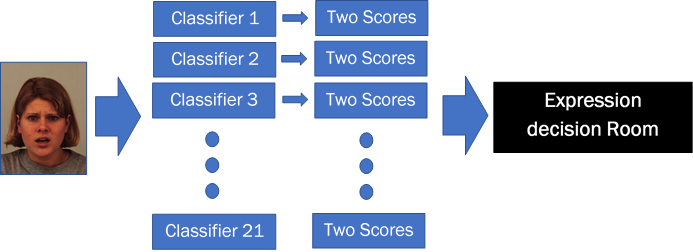
\includegraphics[width=.7\textwidth]{Chapter4/Figs/21Class.png}
%  \caption{21-Pairwise classifiers    \label{fig:21-Pairwise}}
%\end{figure}
%
%\begin{figure}[H]
%  \centering
%      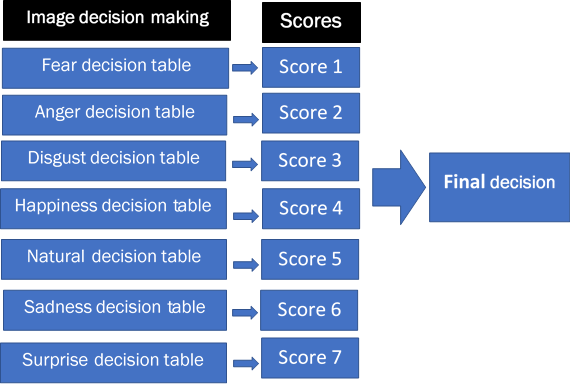
\includegraphics[width=.7\textwidth]{Chapter4/Figs/decision_room.png}
%  \caption{Seven specialized classifier groups      \label{fig:Seven_specialized}}
%\end{figure}
%
%
%
%
%%\section{Pairwise classification effects}
%\begin{figure}[H]
%  \centering
%      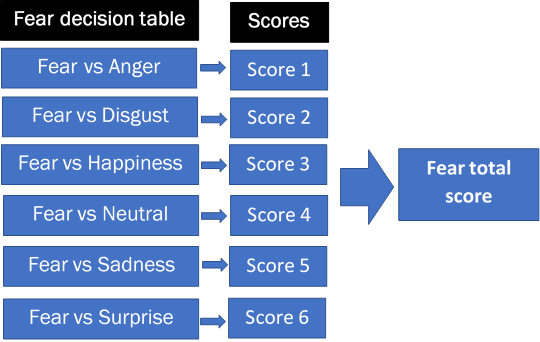
\includegraphics[width=.7\textwidth]{Chapter4/Figs/decision_table.png}
%  \caption{Two groups classification level     \label{fig:newLayer}}
%\end{figure}
%


%\begin{table}[H]
%\centering
%\caption{Normal
%Confusion matrix with 0.898 overall accuracy}
%\label{OldConfusion}
%\begin{tabular}{|l|c|c|c|c|c|c|c|}
%\hline
%\multicolumn{1}{|c|}{} & \textbf{Fear}  & \textbf{Anger} & \textbf{Disgust} & \textbf{Happy} & \textbf{Neutral} & \textbf{Sad}   & \textbf{Surprise} \\ \hline
%\textbf{Fear}          & \textbf{0.671} & 0.143          & 0.043            & 0.000          & 0.000            & 0.143          & 0.000             \\ \hline
%\textbf{Anger}         & 0.000          & \textbf{0.857} & 0.071            & 0.000          & 0.000            & 0.071          & 0.000             \\ \hline
%\textbf{Disgust}       & 0.000          & 0.043          & \textbf{0.929}   & 0.000          & 0.000            & 0.029          & 0.000             \\ \hline
%\textbf{Happy}         & 0.000          & 0.000          & 0.000            & \textbf{0.986} & 0.014            & 0.000          & 0.000             \\ \hline
%\textbf{Neutral}       & 0.000          & 0.000          & 0.000            & 0.014          & \textbf{0.986}   & 0.000          & 0.000             \\ \hline
%\textbf{Sad}           & 0.043          & 0.029          & 0.043            & 0.000          & 0.000            & \textbf{0.886} & 0.000             \\ \hline
%\textbf{Surprise}      & 0.014          & 0.000          & 0.014            & 0.000          & 0.000            & 0.000          & \textbf{0.971}    \\ \hline
%\end{tabular}
%\end{table}























%\subsection{The Karolinska Directed Emotional Faces (KDEF)}
% To evaluate our proposed method,  we used a common database called KDEF (The Karolinska Directed Emotional Faces), figure \ref{fig:CH3KDEF} shows some samples for it. KDEF contains a total set of 4900 pictures of human facial expressions of emotion. The material was developed in 1998 by Daniel Lundqvist, Anders Flykt and Professor Arne Öhman at Karolinska Institutet, Department of Clinical Neuroscience, Section of Psychology, and Stockholm, Sweden \cite{lundqvist1998karolinska}. The set contains 70 individuals, each displaying seven different emotional expressions, each expression being photographed (twice) from five different angles. In our experiments with KDEF, we used only frontal faces, which means 70 images for each facial expression, 490 images in total. 
%
%%%%%%%%%%%%%%%%%%%%%%%%%%%%%%%%%%%%%%%%%%%%%%%%%%%%%%%%%%%%%%%%%%
%\begin{figure}[H]
%\center
%  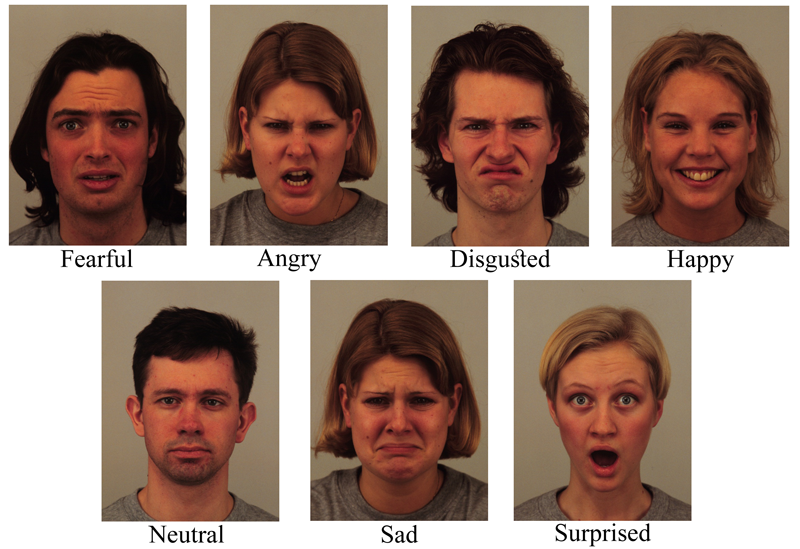
\includegraphics[width=0.5\textwidth]{Chapter3/Figs/KDEF.png}
%    \textbf{\caption{Faces samples from KDEF database}\label{fig:CH3KDEF}}
%\end{figure}
%%%%%%%%%%%%%%%%%%%%%%%%%%%%%%%%%%%%%%%%%%%%%%%%%%%%%%%%%%%%%%%%%%


%
%\subsection{KDEF and emotion in the wild comparison}
%All proposed methods work with images have been produced from actors, so most of the expressions are not real. Moreover, the ways real people express their emotions are varied and changeable from one to one, and sometimes from one ethnicity to another, especially with fear, sad, surprise and anger. So, this creates a real challenge for us.



%____________________________________ Pairwise selection _____________________________________%




%\clearpage
%
%\newpage

\section{Summary}
\label{sec:ch4_Summary}
Rather than using a single type of texture descriptor for appearance-based classification of emotions, we showed that a combination of LBP, HOG and D-SURF significantly increases classification accuracy. Furthermore, the random forest's feature selection was used to empirically identify the important regions of the faces for classifying emotion.  As might be expected these are mainly around the eyes, mouth, creases on either side of the nose and the forehead.  Use of our empirically defined importance mask enhances classification accuracy.

Further improvements to classification accuracy were obtained by pairwise weighted voting between dichotomous classifiers, and we showed how to learn optimal weights using an evolutionary algorithm.  The resulting accuracies are significantly better than the current published state of the art results on the posed KDEF data. Nonetheless, particularly for unposed data, classification of fear, anger, disgust, sadness and surprise remains imperfect, and we obtain classification accuracies of about 77\%. We observe that these are the emotions that humans find more difficult to classify from static images in the eLFW data.  
